\chapter{Language family, neighbors and previous work} % Main chapter title
\label{ChapterContext} % Change X to a consecutive number; for referencing this chapter elsewhere, use \ref{ChapterX}

\ea
\gll juu va m=e=juu saxhuti nyakoo-vwe i=jaxhut ko i=vamale...\\
 real too.much \gl{subr}=1\gl{sg}=real narrate for-2\gl{pl} \gl{def}.\gl{sg}=story about \gl{def}.\gl{sg}=Vamale\\
 \glt \qu{It is beyond me to properly tell you the story of the Vamale language...}
\z

This chapter aims to introduce Vamale in its genealogical context, as well as its current geographical environment. The language has been affected by its role in the area over time, its neighbors, and the contact situations born of that. Because Vamale speakers were one of the most severely impacted speaker communities of the 20th century in New Caledonia (see \chapref{chap:Tipije}), \textit{i vaa can vije}, the 1917 Kanak revolt or war, plays a crucial role in understanding why so few speakers remain, and why Vamale is a pluricentric language spoken by traumatized people. \chapref{chap:Tipije} summarizes the background and main events of this war.

Vamale is said to have approximately 100 speakers left \parencite{eberhard_vamale_2020}. Asking community members to list everyone capable of having a conversation in 2017 yielded 186 names, nine of whom have since passed away (as of January 2021). Worryingly, only 32 speakers are younger than thirty, and only 2 are minors. Most fluent speakers are over 60 years old. Though the language is used in ceremonies and some households (e.g. Téganpaik chief's house), and amongst many adult speakers, persons under 25 years of age barely use it with each other. A notable exception is the village We Hava, where a majority of residents understand, and many speak, the language. In one, maybe two generations, the language will stop being spoken, unless the trend is reversed. 
%The cultural focus on older males also reflects on the speaker census. When asked, most (male) speakers claimed that the women and children did not really speak it, which turned out to be an exaggeration. 81 of 180 speakers counted by a community member were women, though exogamous practices mean that they rarely stay in the village after marrying. 
On a hopeful note, an association was founded in 2019 with the goal of maintaining the language vital and promote its use (pictured in \Cref{fig:assoc}). Several workshops to this end have already taken place since the beginning of the research project, like the one shown in \Cref{fig:workshop}.

\begin{figure}
	\centering
		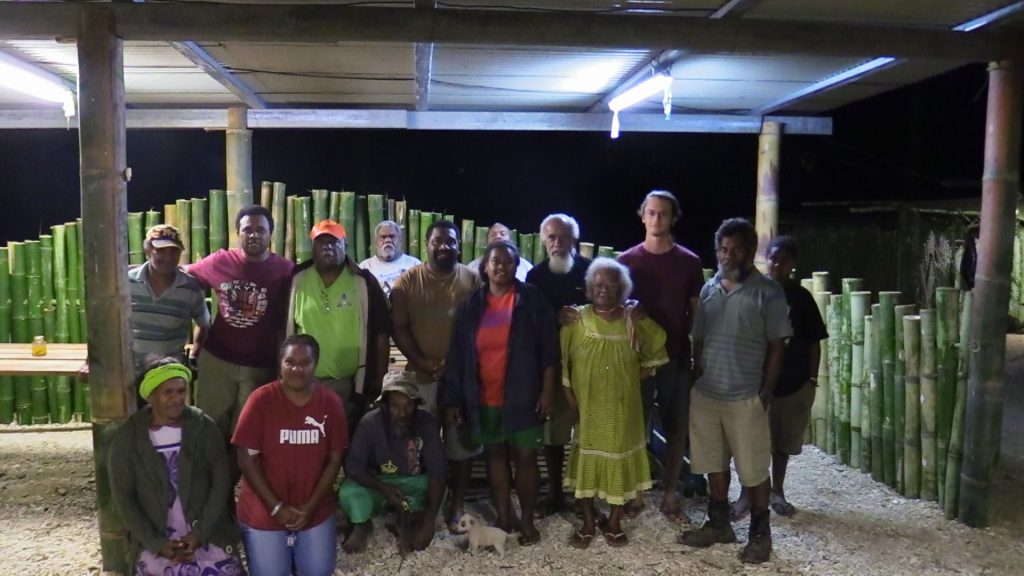
\includegraphics[width=\linewidth]{figures/assoc}
		\caption{The founding members of the Association Vamale.}
		\label{fig:assoc}
\end{figure}

	\begin{figure}
	\centering
	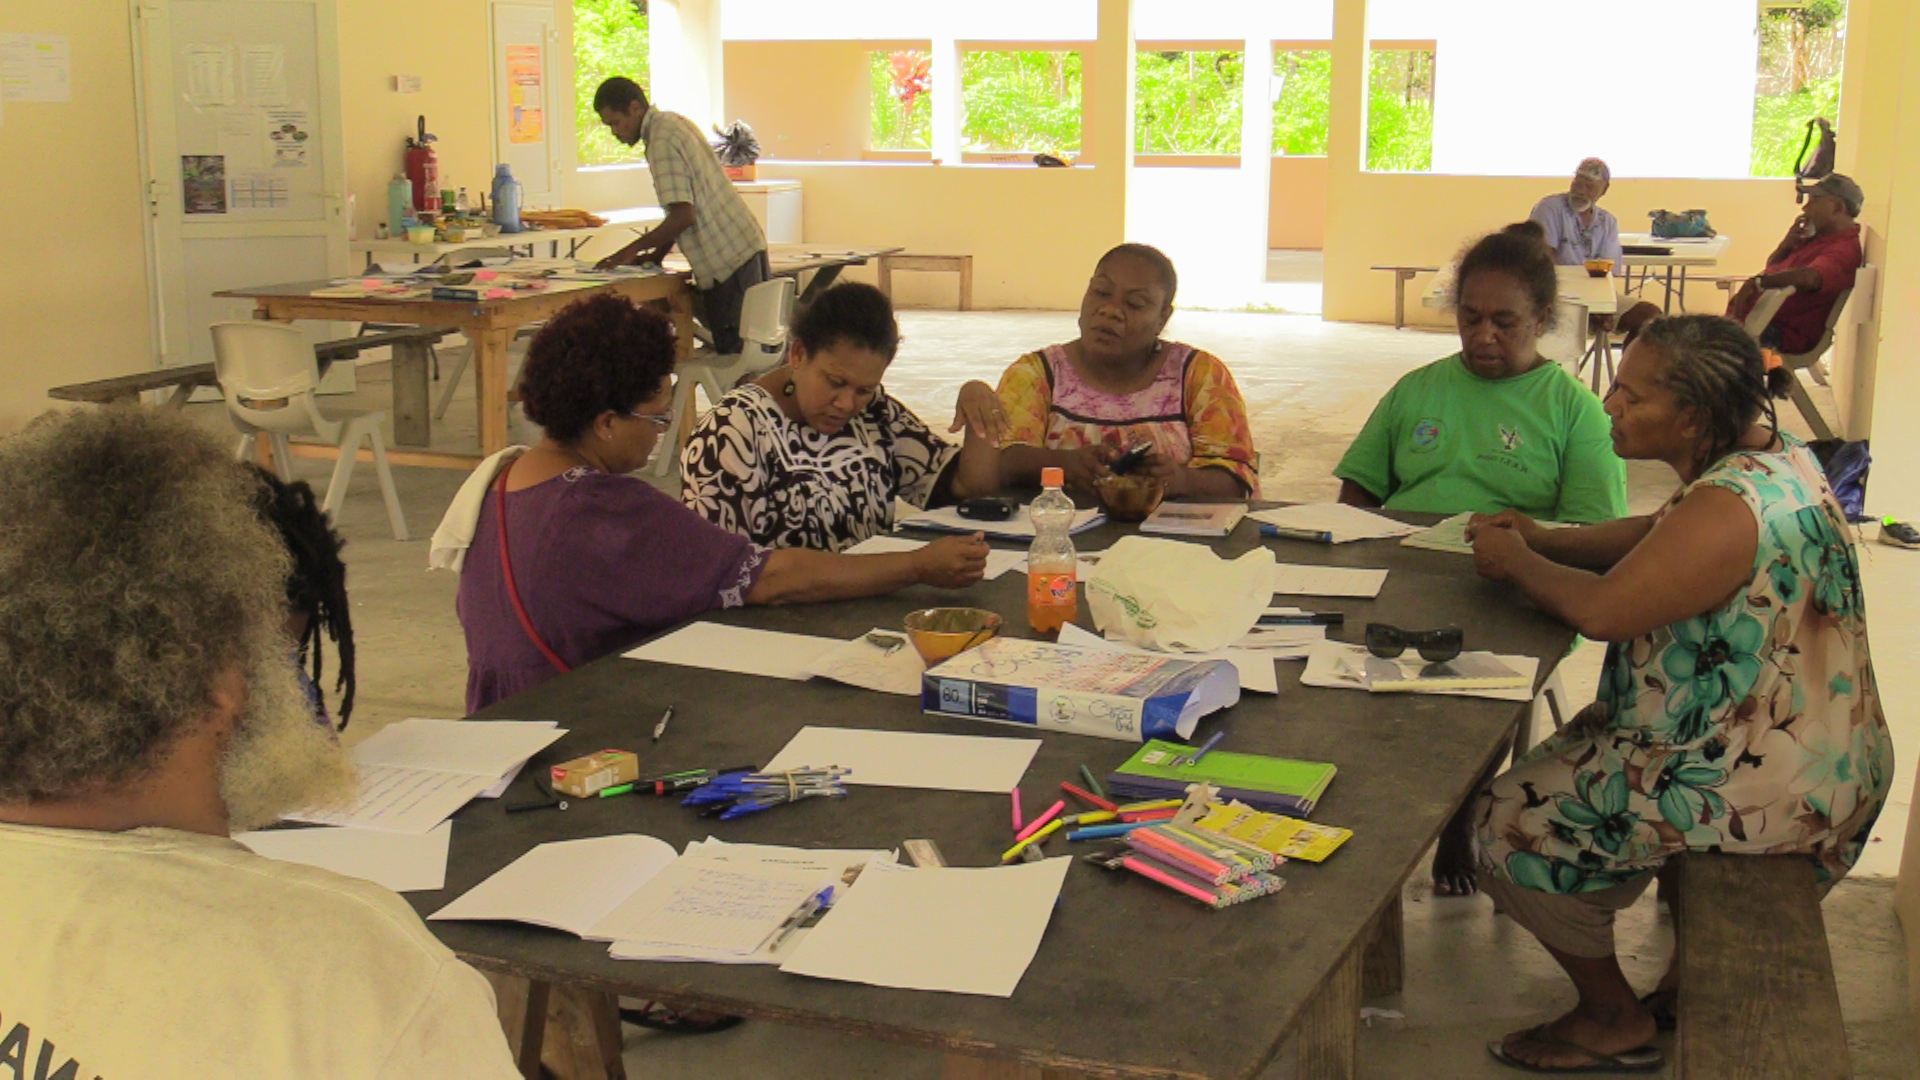
\includegraphics[width=\linewidth]{figures/atelier}
	\caption{A language workshop in late 2018, with members of the Academy of Kanak Languages.}
	\label{fig:workshop}
\end{figure}

%The chapter is structured as follows: first, the language is situated in the world (\Cref{sec:place}). The language's place in its family is discussed in \Cref{sec:Ling_Profile}. Previous work on the language is listed in \Cref{sec:prev_work}. \Cref{sec:Tipije} summarizes the events surrounding the war of 1917, while \Cref{ssec:Frenchpolicy} describes the circumstances leading to the language's decline after the displacement of the speakers. The section following this describes the situation of the language today: the villages in which it is spoken (\Cref{ssec:Geo}), the society which uses it (\Cref{ssec:Soc}), the cultural context relevant to language transmission (\Cref{sec:CultContext}) and code-switching (\Cref{sec:Multiling}), as well as Vamale's linguistic neighborhood (\Cref{ssec:neighbors}). The issue of the language's name is discussed in \Cref{sec:LanguageName}. A section on the main consultants introduces the work group and their linguistic background (\Cref{sec:Consultants}). The project's methods of data gathering are described in \Cref{sec:Meth}. Some information regarding doing fieldwork in New Caledonia closes the chapter (\Cref{sec:Field}).
 This section describes the situation of Vamale today. Below are brief descriptions of the villages in which most speakers live (Nouméa, the capital, is exempt), and a list of the languages found in the direct vicinity of Vamale. %The latter is important in the context of the name of this work's subject, and whether it is a dialect or not (see \sectref{sec:LanguageName}).


\section{Current geographical location of Vamale}
\label{sec:place}
Vamale is spoken on the northeastern coast of \textit{Grande Terre}, the biggest island in the archipelago of New Caledonia (\Cref{fig:SouthOceanic}). These islands, located south of Vanuatu in the subtropical Coral Sea, were settled around 3,200 years ago by Lapita sailors from Vanuatu \parencites[334]{lynch_efate-erromango_2004}[309]{sand_what_2007}. Contacted in 1774 for the first time by Europeans, the archipelago was formally claimed by the French in 1853, to break up British dominion in the area. French settlement, and the plantations tied to it, led to an influx of speakers of Vietnamese, Polynesian, Vanuatuan, and French varieties. Before this period, the islands hosted a family of at least 35 South Oceanic varieties\footnote{Leenhardt described 36 varieties, some of which are considered dialects of the same language, e.g. Orowe, Hamea, and Ajië. Given that in the 1940s, many of them were already quasi-extinct (e.g. Waamwang, Arhâ, and the ceremonial varieties of Drehu and Nengone), and given the catastrophic decline of the Caledonian population, \textit{and} how many small languages still co-exist in the North, a larger number may be presumed to have existed.} as well as a Nuclear Polynesian language spoken on Iaai/Uvea since the 17th century: Fagauvea (see \Cref{fig:SouthOceanic})
Vamale is the only member of the Voh-Koné linkage situated on the rainy east side of the central mountain range, about 375 km northeast of the capital Nouméa. The sea immediately to the east, and steep, sparsely populated mountains to the west mean that there is an about 5km large belt in which humans live in any density to speak of, and where Kanak languages are mostly found nowadays. Vamale is spoken in an area approximating 25 km\textsuperscript{2}, but apart from isolated houses like Laurient Gohoupe's far upstream of We Hava, the speakers can be found in five villages (and, of course, the bigger towns of the territory). These will be described in more detail in \sectref{ssec:Geo}.


\label{ssec:Geo}
%\begin{figure}
%	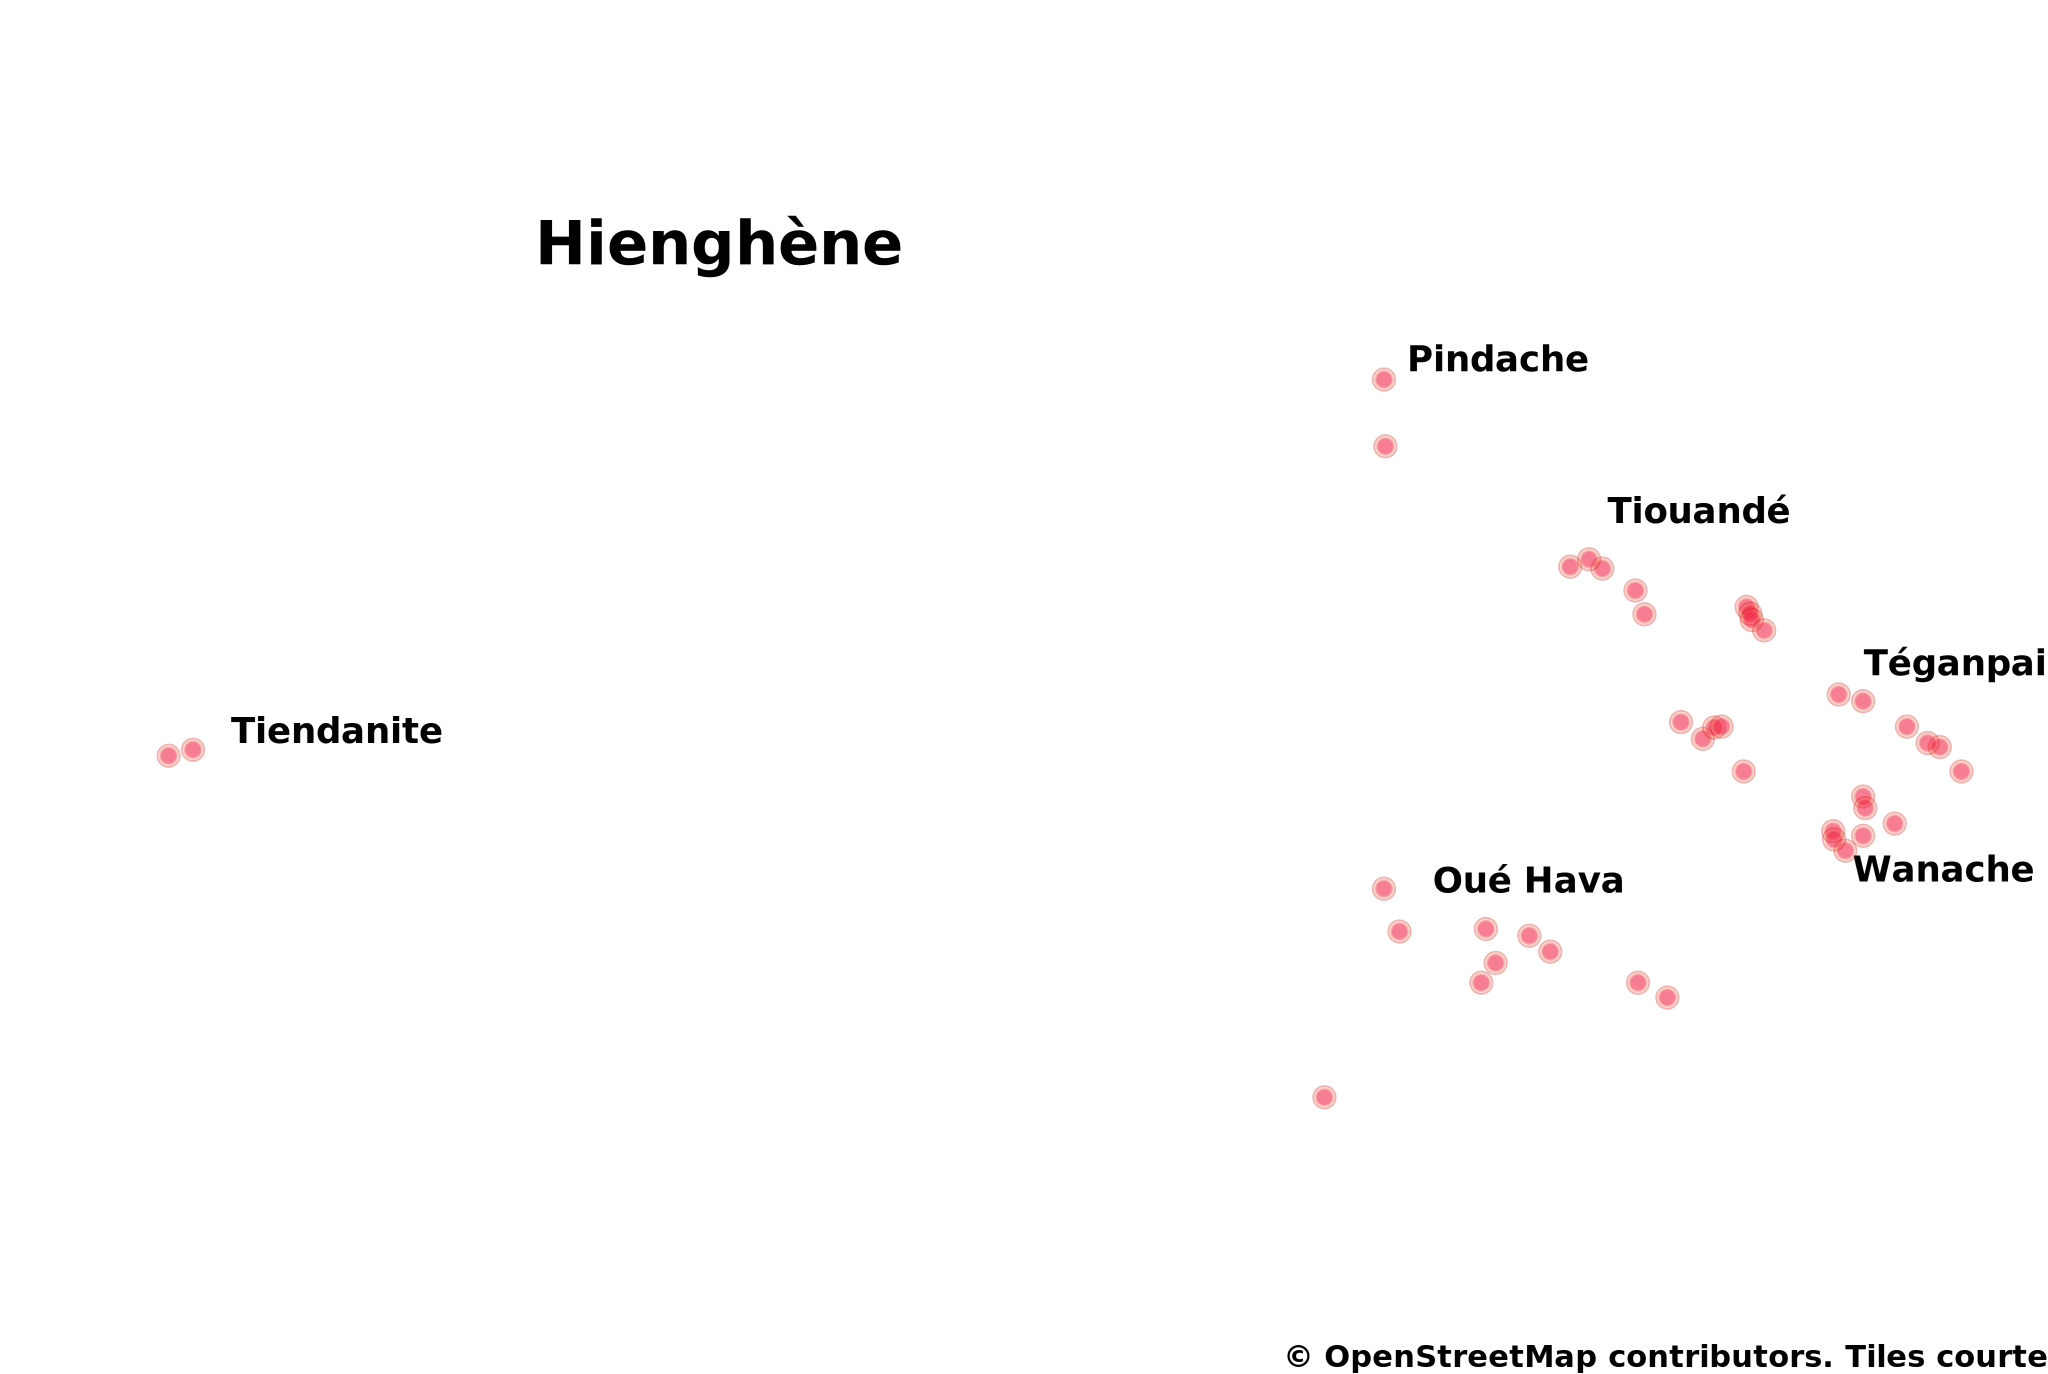
\includegraphics[width=15cm]{figures/map_dots}
%	%Gouvernement de la Nouvelle-Calédonie, 22-11-2017
%	\caption{Approximate map of speaker households on the east coast (Government of New Caledonia, 22.11.2017), dots are my own, thanks to Florian Matter.}
%	\label{fig:speakerMap}
%\end{figure}



%This documentation will produce one of the bigger corpora on New Caledonian languages, and may be a useful source in researching variation across time and space. For example, we have little knowledge of the history of Voh-Koné languages. Since they are concentrated between Voh and Koné on the east coast, and Vamale used to be spoken in the mountains, it is likely that they first settled in the mountains and then crossed them to the other side, but what the relation between the languages is, how and when they moved, and what the precolonial history of the area is, are questions more easily answered with comprehensive records of oral history, borrowings, and toponyms.
Vamale is spoken in several villages in the communes of Touho and Hienghène along the east coast of northern New Caledonia, in some villages in the mountains, and perhaps close to the west coast (Baco, Koné). The community is thus relatively widespread, which has given rise to a number of “family idioms”.
The Vamale-speaking area is large but sparsely populated, and concentrates on four villages. This work will usually prefer the word ``village" to ``tribe", which would be the translation of the official French term \textit{tribu}, because the Vamale word used for village, \textit{xhoogo}, means \qu{home} and has no connotation of a tightly-knit group of clans (especially since the 1917 war), and because it ultimately derives from a colonial vocabulary trying to establish a fundamental difference between Kanaks and settlers.
This section will thus describe the villages in which Vamale is spoken. 

\begin{figure}
	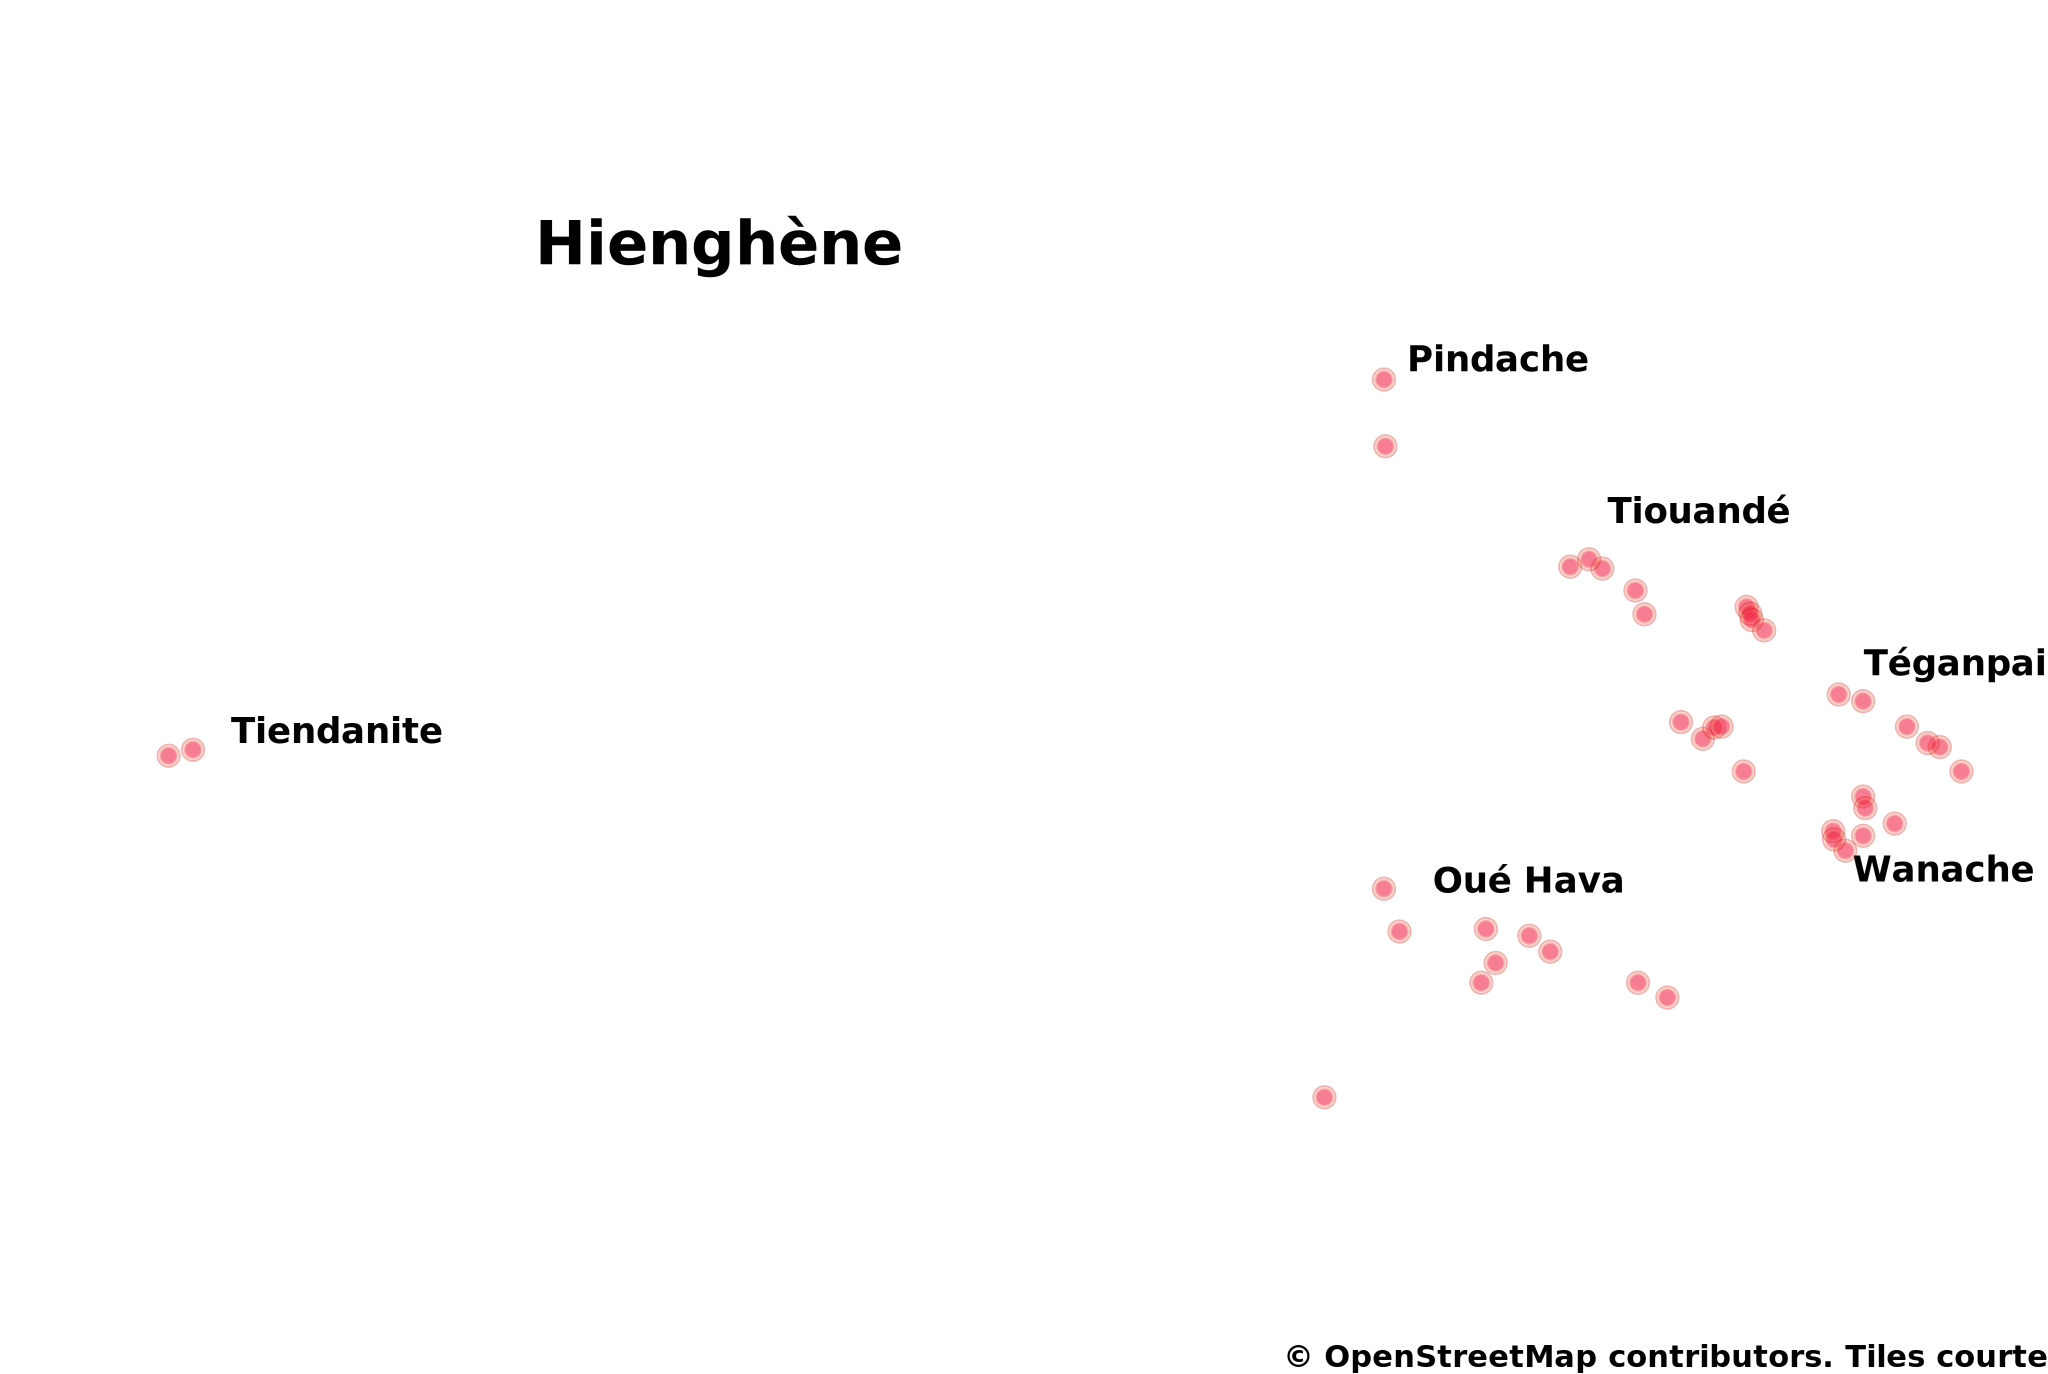
\includegraphics[width=\linewidth]{figures/map_dots.pdf}
	\caption{Map of speaker households. Approximate map of speaker households on the east coast (\citeauthor{gouvenementdelanouvelle-caledonie_explorateur_2019}, 2017-11-22), dots are my own, thanks to Florian Matter.}
	\label{map:dots}
\end{figure}

\subsection{Téganpaïk}
\ort{Téganpaïk}, or in Pije [tʰeᵑgane ˈpaːik] \qu{split stone}, after a placename close to the cemetery, is a village of about 200 inhabitants. Haudricourt translates the name as \textit{tnek-ngen-paik} \qu{oven-in-stone} \parencite[229]{haudricourt_langue_1968}.%The chieftaincy is held by a Oué man, but traditionally belongs to the Néa clan. 
A Shell gas station, a community center and a church are the only public buildings; the closest school is in Cèmuhî-speaking Touho, though many children go even further to Paicî-speaking Poindimié for secondary education. Téganpaïk is the biggest Vamale-speaking village, and the research project was based there. Traditionally Pije, many families are bilingual, and old marriage alliances have brought women speaking other languages as well. In most families, Kanak language transmission stopped around 1990. %almost all of my first, exploratory field trip there, with members of the Pei family.
The village is a string of houses along the national road RN1 and squeezed between steep mountains and the sea (there are rarely more than 100 metres between them). While the pre-contact population of the fertile Tipije (Pij. \textit{ti pije} \qu{estuary snare}, the Pije name for the river itself is \textit{le pije} \qu{in snare}), and Tiwaka valleys, was likely large, this coastal strip harbors no fields and few fruit trees, and may not have been as densely populated before the arrival of Vamale speakers. Almost beachless, and facing sharp, mostly dead coral at low tide, Téganpaïk does not attract many tourists, and with a chiefly ban on kava bars,\footnote{The next village to the East, \ort{Kongouma} (Cèm. /ko-goo-mwa/ \qu{on the wall}), sports three \textit{nakamals} and kava drinkers come from Hienghène and Touho to lift \textit{sels}.} the only points of interest to travelers are the Shell gas station and a picknick area near the sea. Touho has a diving school and boats one can rent, whereas the only bigger boat the village had, the \textit{Dongan}, was lifted and crashed on the other side of the road by cyclone Betty in 1995. This disbanded the fishing cooperative that had begun between villagers, and the boat's low-tide haven, a pool created by coral blocks, is now used for swimming and as a sardine reproduction sanctuary. Cyclones are becoming stronger almost every year, and with warmer, more acidic waters, the coral barriers protecting Grande Terre against the occasional tsunamis and other high waves are deteriorating. Villagers have begun planting mangrove trees to attract fish and crabs, but also as a protection against coastal erosion and waves. The author did not meet anybody unworried about climate change.

Téganpaïk is a tightly-knit community. Its children play together, the men go hunting on horseback and in pickup trucks and fish on bamboo rafts and in motorboats. The protestant church is an important center to the community, and one of the main domains of Vamale.
Téganpaïk's clan council also administrates Wanaa (see \sectref{subsec:Wanaa}) as well as the former leper colony Mahena/Ma\"ina, which is composed of few houses and can be considered a suburb of Téganpaïk.

\begin{figure}
	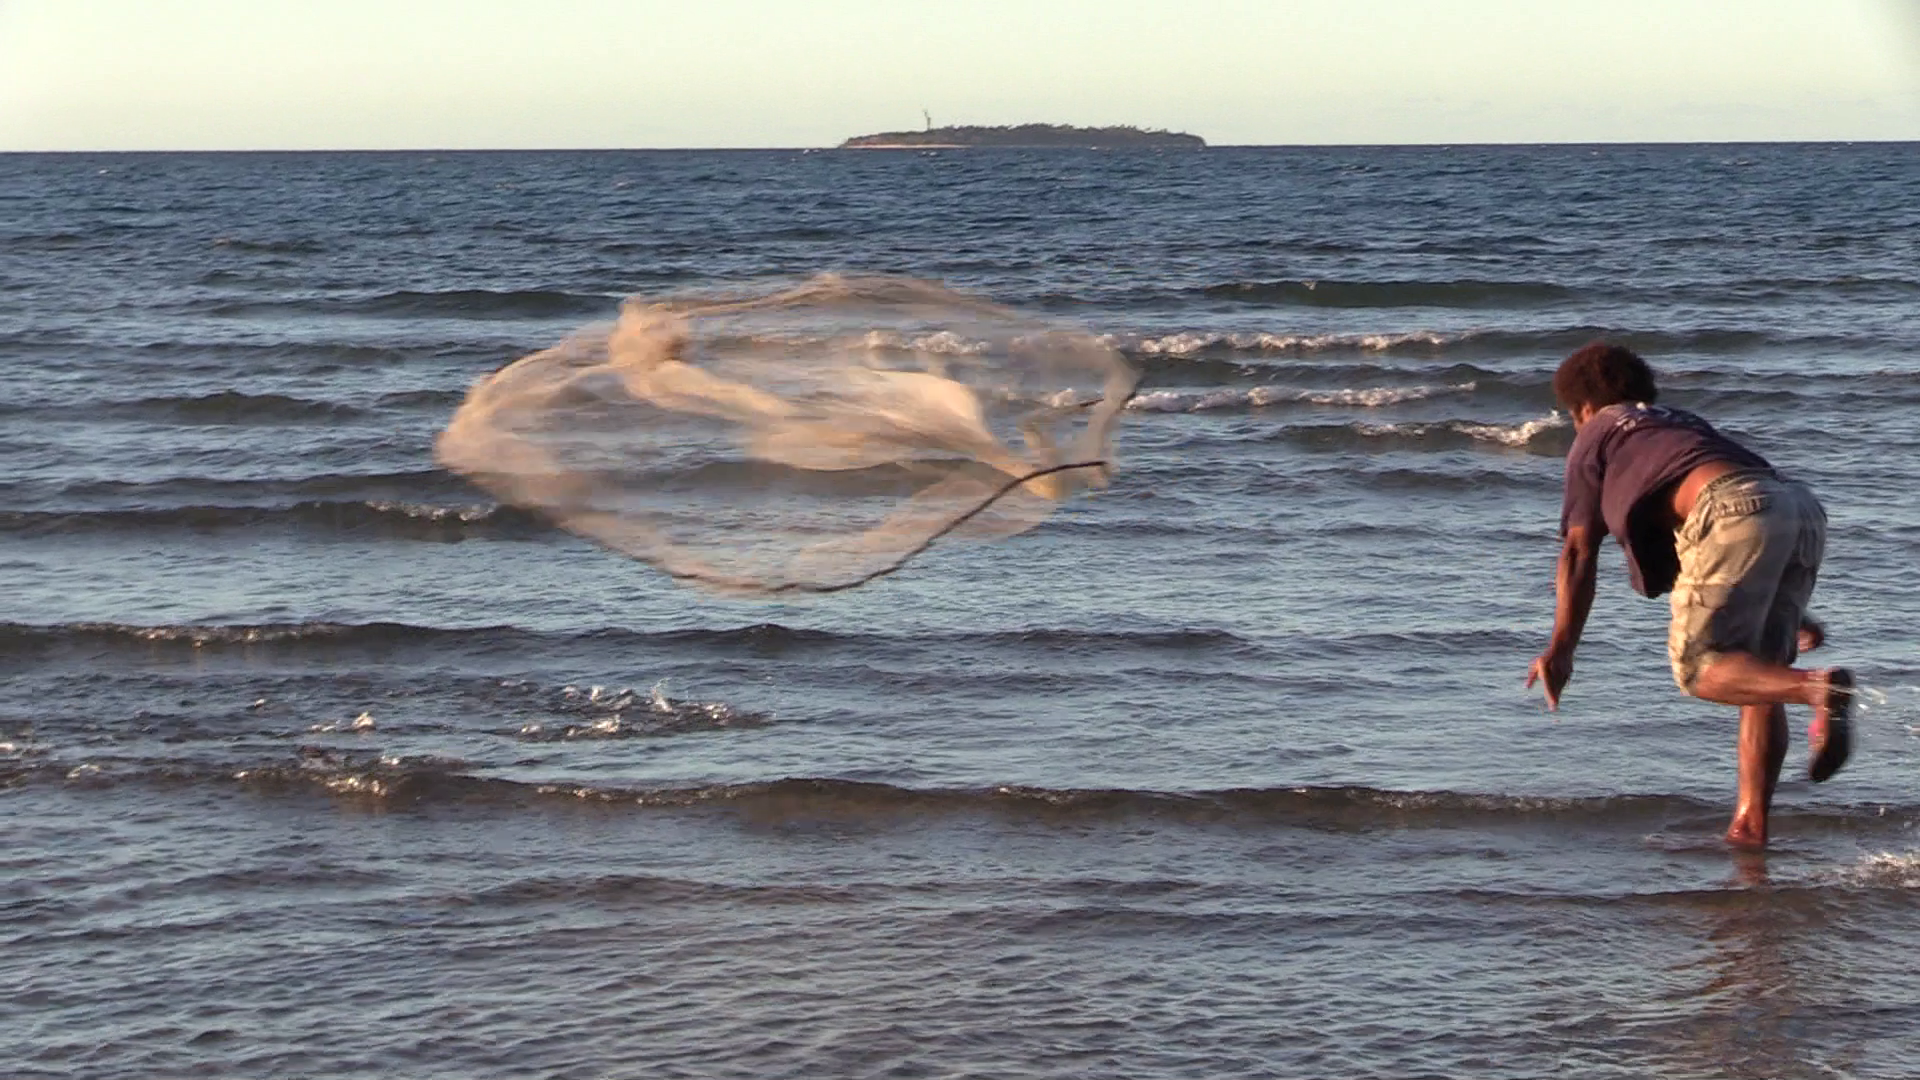
\includegraphics[width=\linewidth]{figures/net}
	\caption{Mr.\ Christophe Pei fishing for sardines in Téganpaïk}
\end{figure}

\subsection{Wanaa}
\label{subsec:Wanaa}
\ort{Ouanache} [wãˈnãː]\footnote{According to inhabitants, possibly from Pije \textit{hwada} \qu{planting spot} \parencite[106]{haudricourt_dictionnaire_1982} or Vamale \textit{(e-)wanaa} \qu{dispute}.} has only 11 houses, but fluent child speakers of Vamale, and many fields belonging to Téganpaïk inhabitants. %Dui's biological mother lives here.
Wanaa was Pije-speaking before 1917, but is now one of the biggest speaker-centers of Vamale. Contrary to Téganpaïk, it is an official tribe, though its chief Luc Oué resides in the former village. A war location in 1917, it welcomed some of the inland refugees.
The village concentrates in two road loops close to the neighboring villages Téganpaïk and Tiouandé, but the tribal grounds stretch south-east following a valley shown in \Cref{fig:wana} until a mountain pass leads to Poyes (see \chapref{chap:Tipije}).
Considering that some of its uninhabited mountain flanks show remains of taro terraces, and that planted araucaria trees can be seen much further upstream, the settling of youths in the wild backyard of the village, Tanaka, is more a reclaiming of former living grounds than a human invasion.

\begin{figure}
	\centering
	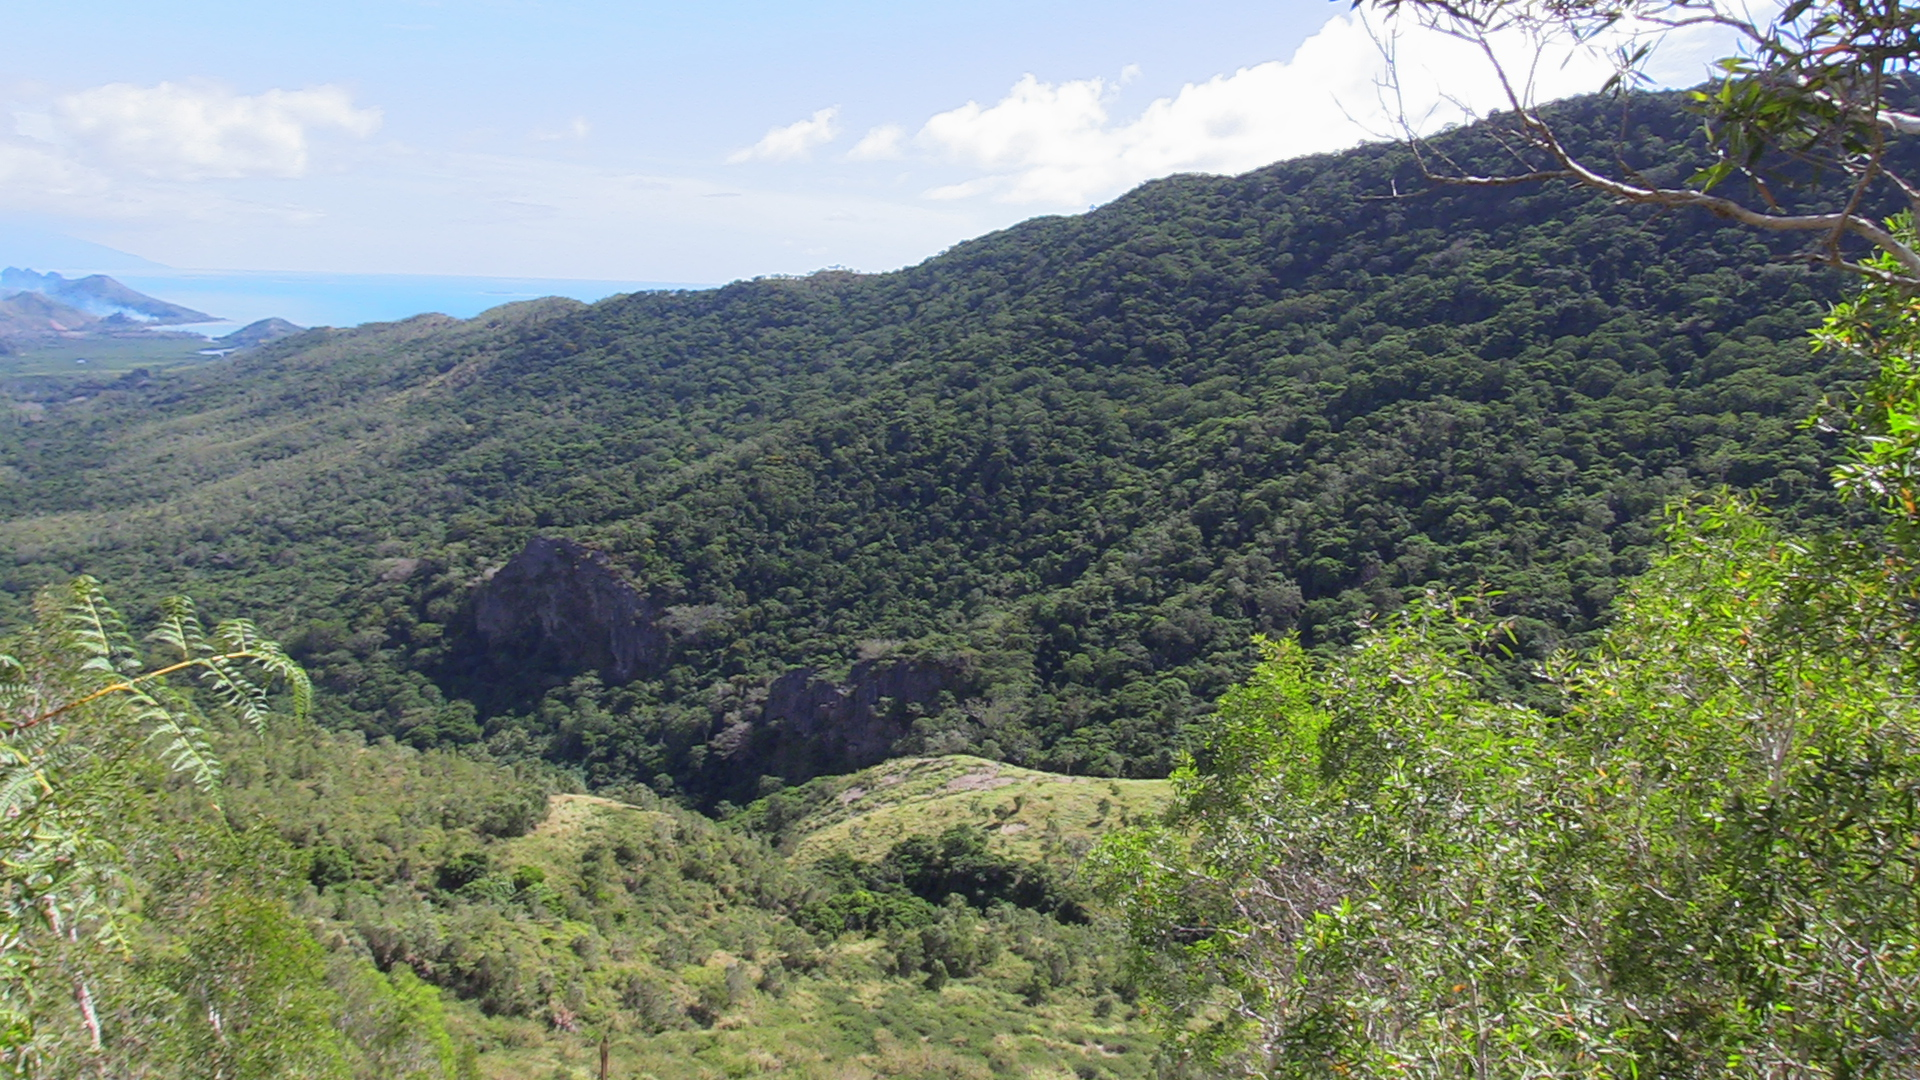
\includegraphics[width=\linewidth]{figures/wanaa}
	\caption{The Kacabwec valley leading to Wanaa. Only part of it is inhabited now.}
	\label{fig:wana}
\end{figure}

\subsubsection{Tiouandé}\largerpage[2.25]
\ort{Tiouandé} (Pije [tʰeˈxʷaːⁿde] \qu{rock garden}) borders the Tipije river on its northernmost end, the sea on the northeastern side, steep mountains and rock formations like ``Napoleon's hat" (Vam. \textit{vaci that} \qu{wind's nucleus}) on the west (shown on the left in \Cref{fig:twd}), and the hill Kapohiyoak (``children-making place") %suffering from deforestation-induced erosion 
which separates it from Téganpaïk. Tiouandé is the village with the most Pije speakers in the region, and is in close and active contact with Téganpaïk. Its chieftaincy is held by the Kalène clan, though the Bwiyâ have held it until the current chief took over. %\textit{fuâ bonu} \ort{Fouan Bonou} and her son \textit{nigai} (\ort{Ningaille}) live there.

\begin{figure}
	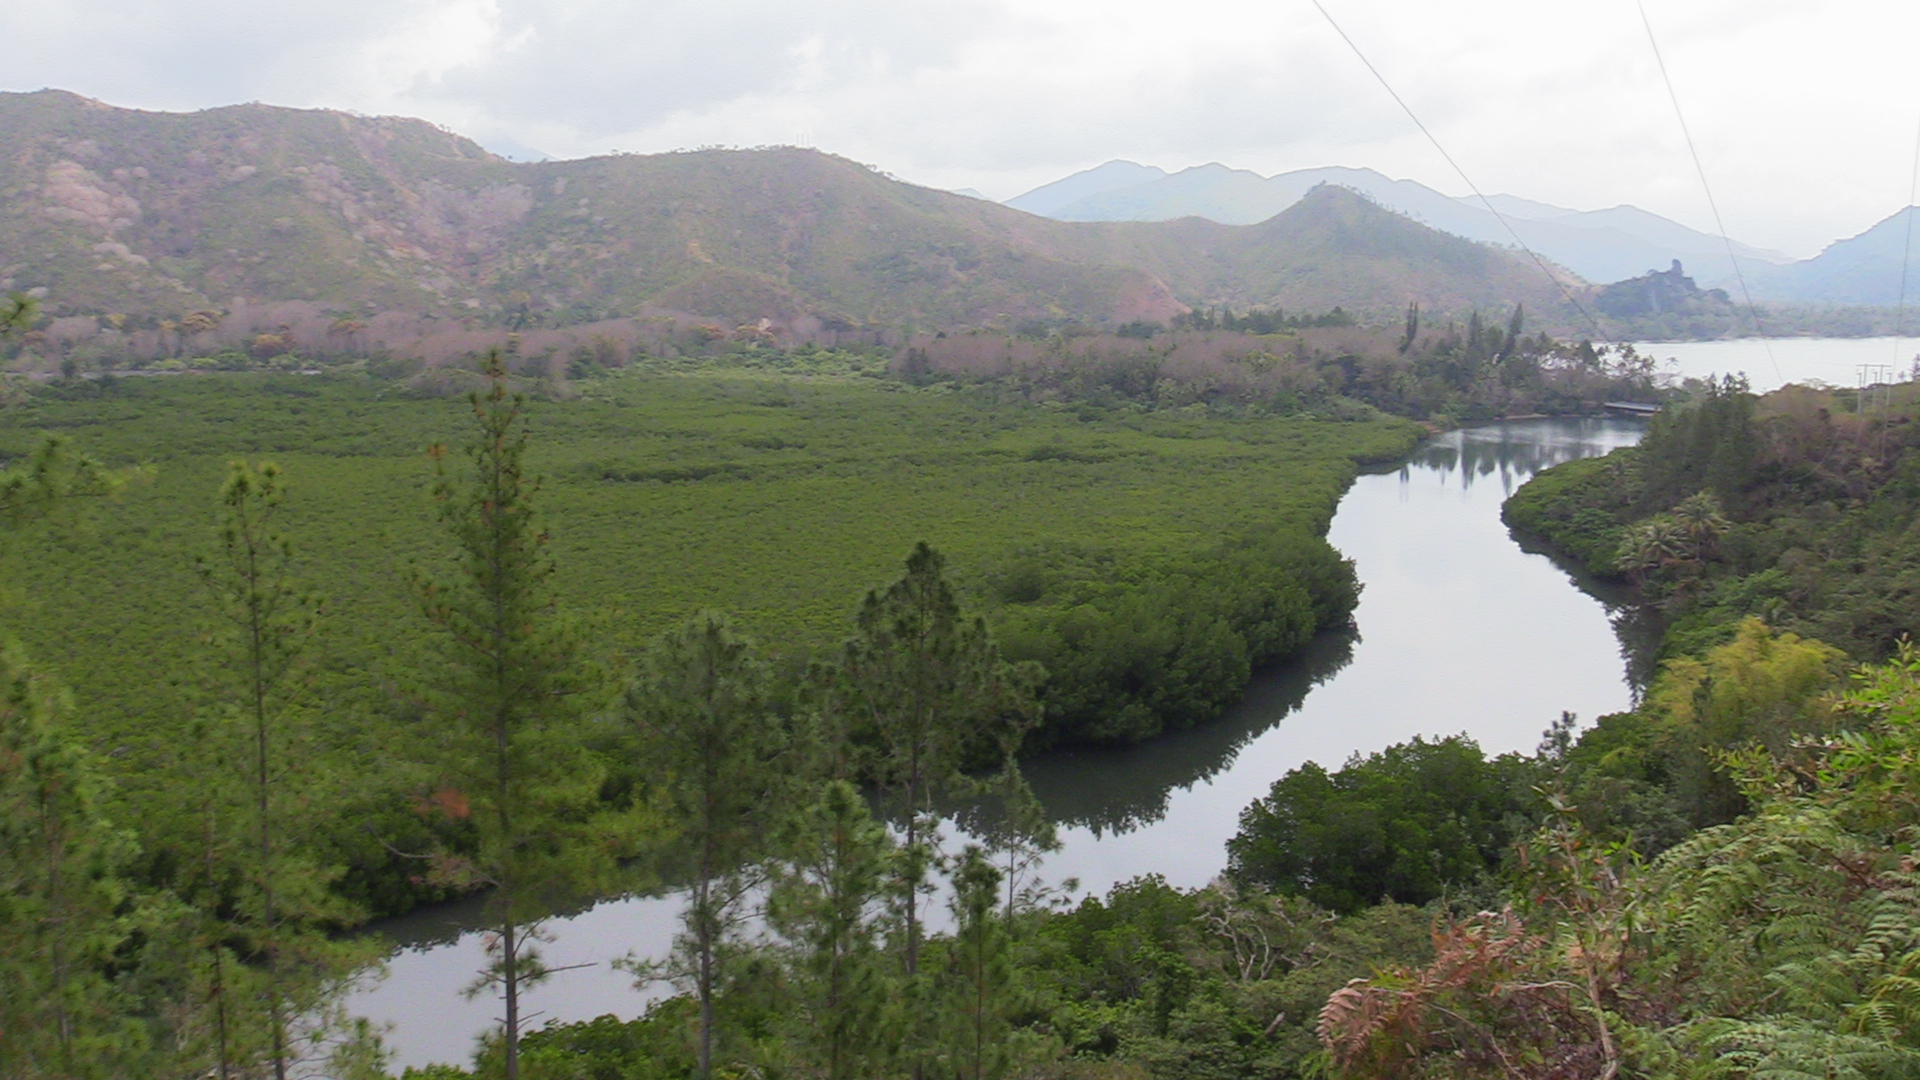
\includegraphics[width=\linewidth]{figures/twd}
	\caption{The Tiouandé estuary}
	\label{fig:twd}
\end{figure}

\subsection{We Hava}\largerpage[2]
\ort{Oué Hava}, Vam. ['we hava] \qu{\textit{Broussonetia papyrifera}\footnote{Used for its bark to make \textit{tapa} cloth.} creek}, %though some speakers mentioned \qu{ghost creek}, 
built along a tributary of the Tipije river, is a group of settlements, about four or five, each consisting of several huts and small houses. An exception makes a classic colonial building, white and facing the river, which is now inhabited by We Hava's former chief Kaina Fouan. The chieftaincy has returned to the traditional owners, the \ort{Tchéou} /ceu/ clan. The long road to \textit{Cake-O} \qu{scoop, bail out-bamboo}, We Hava's last dwelling and home of the oldest Vamale speaker Philippe Gohupe (the author of the Tipije text in \Cref{text:tipije}), is now bordered by bamboo groves and forest in various states,{\interfootnotelinepenalty=10000\footnote{Burning brush is a problem for local forestry. While careful burns were part of the slash-and-burn agricultural model, unsupervised fires are a common cause nowadays for wildfires, and are universally frowned upon and creates problems for wildlife, water table, and of course botany. The straw needed for traditional thatching is especially vulnerable.}} but all along the road, traces of abandoned villages can be seen on both sides of the river. We Hava and the settlement on the other side, Tipije, are what remains of ca. 14 settlements in the valley.

\begin{figure}
	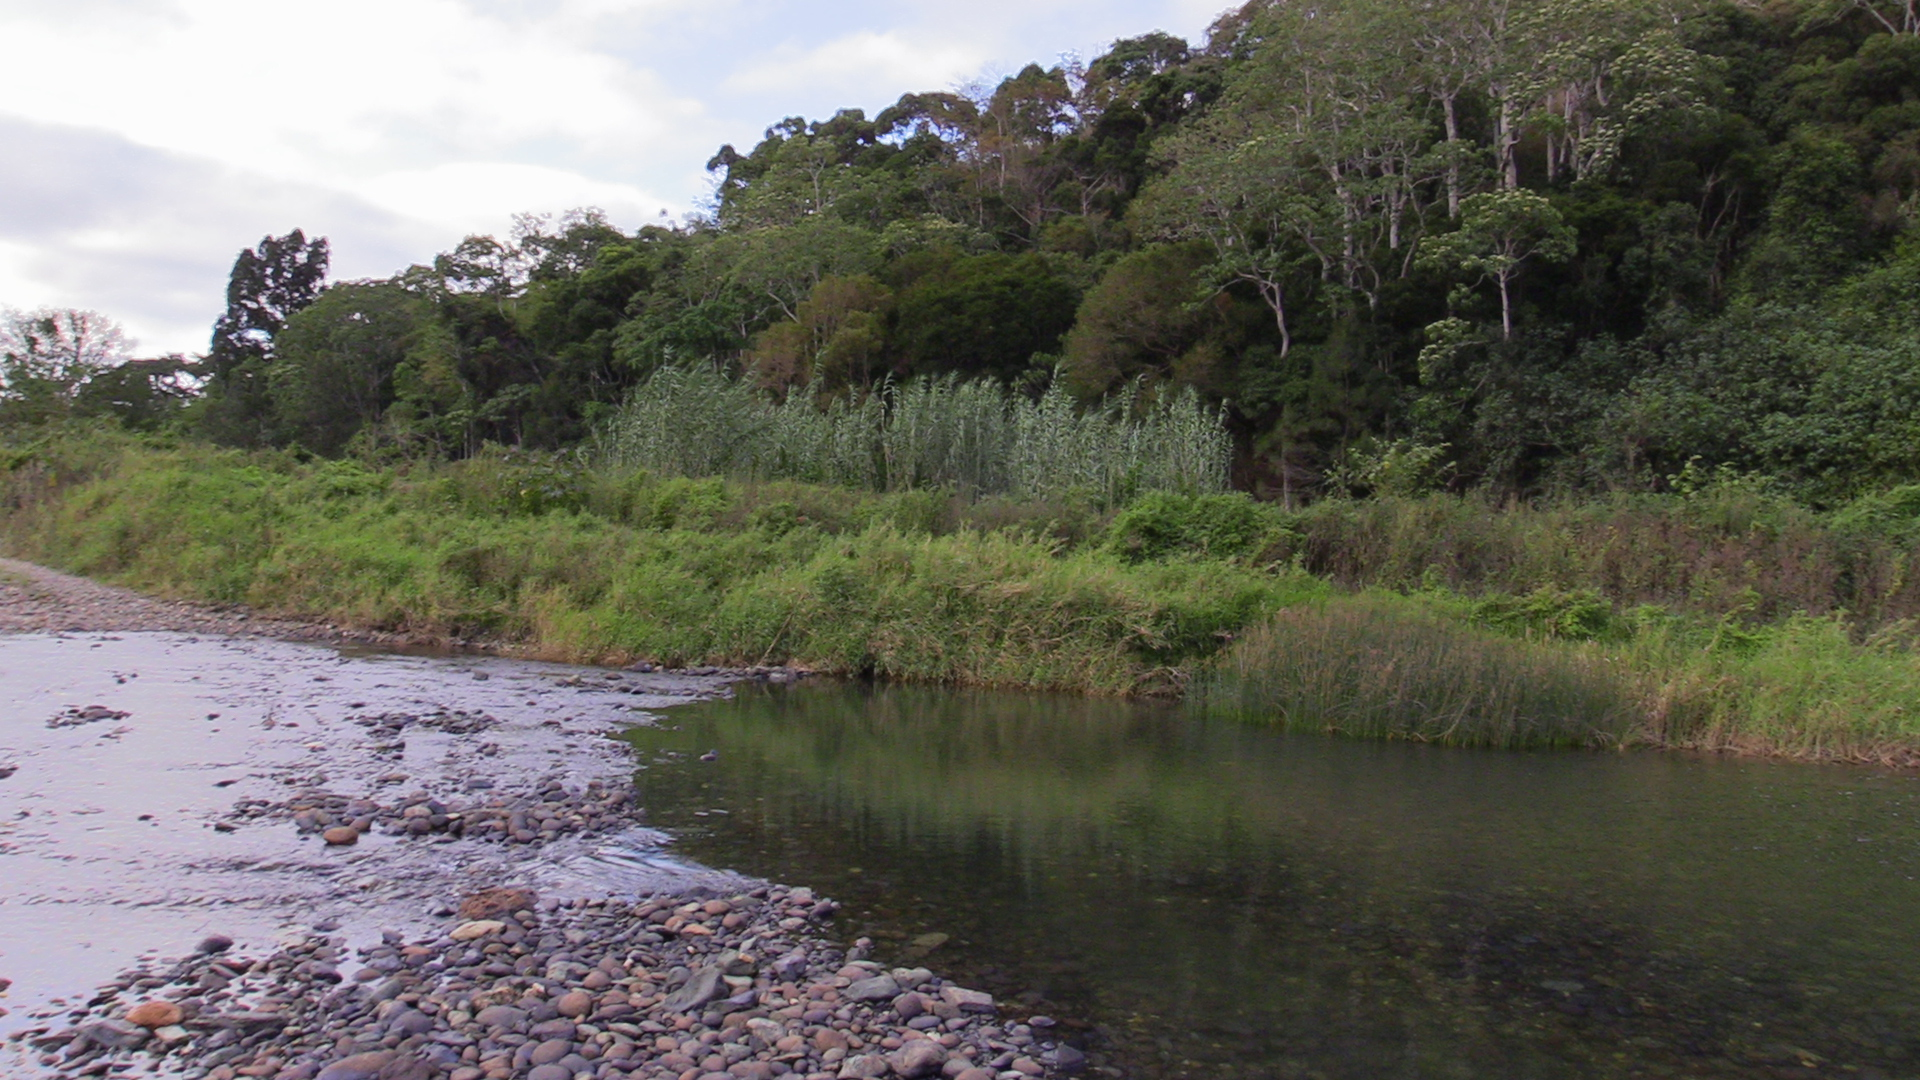
\includegraphics[width=\linewidth]{figures/wehava}
	\caption{The We Hava river}
\end{figure}

\subsection{Tiendanite}
\ort{Tiendanite}, in Vamale ['seːⁿɟan̥it], the home village of the politician Jean-Marie Tjibaou, is buried in misty hills up-stream of a Tipije tributary. It mostly houses eastern Nemi and Mountain Pije speakers, but also three households of Vamale Usa speakers, who are in irregular contact with coastal speakers. Usa is a Voh-Koné variety formerly spoken in a valley tributary to Pamale, and has a half-dozen speakers under 40 years of age. %The daughter is my age and speaks it. 
Children run around speaking Pije. Vamale speakers arrived there after the war \parencite[62]{couhia_pascal_2008}, though their earlier presence is likely. %A beautiful, remote place. 

Having provided a brief overview over the places in which Vamale is spoken, the chapter now introduces some important societal points.

\section{Language family}
\label{sec:Ling_Profile}
\largerpage
%This section is about the genealogical context of Vamale. 
\textcite[112]{lynch_oceanic_2002} classifies the New Caledonian language family and the Southern Vanuatu family as part of the Southern Melanesian family. With South Efate languages, this group forms the Southern Oceanic linkage \parencite[112]{lynch_oceanic_2002}, itself a linkage in East Malayo-Polynesian (see \Cref{fig:SouthOceanic} for a map). \textcite[334]{lynch_efate-erromango_2004} hypothesizes that New Caledonia was settled rather directly from Efate, which would make sense with its status of a family inside a linkage.
Oceanic languages are grouped into innovation-defined groups and innovation-linked ones \parencite[93]{lynch_oceanic_2002}, distinguishing languages which descend from a reconstructible proto-language, from languages that form a group through innovations shared via contact, or where innovations have occurred in overlapping smaller groups. The latter case is much more frequent in this area of the world. 
\begin{figure}
% 	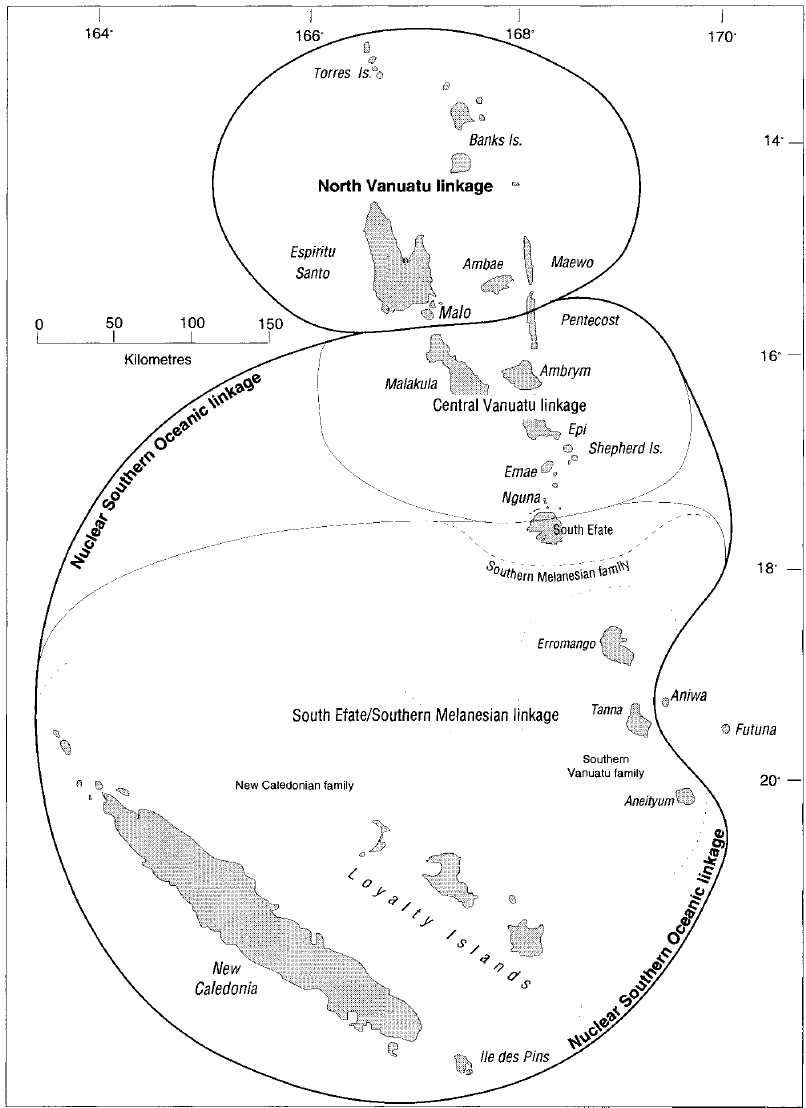
\includegraphics[width=\linewidth]{figures/lynch_south_oceanic}
	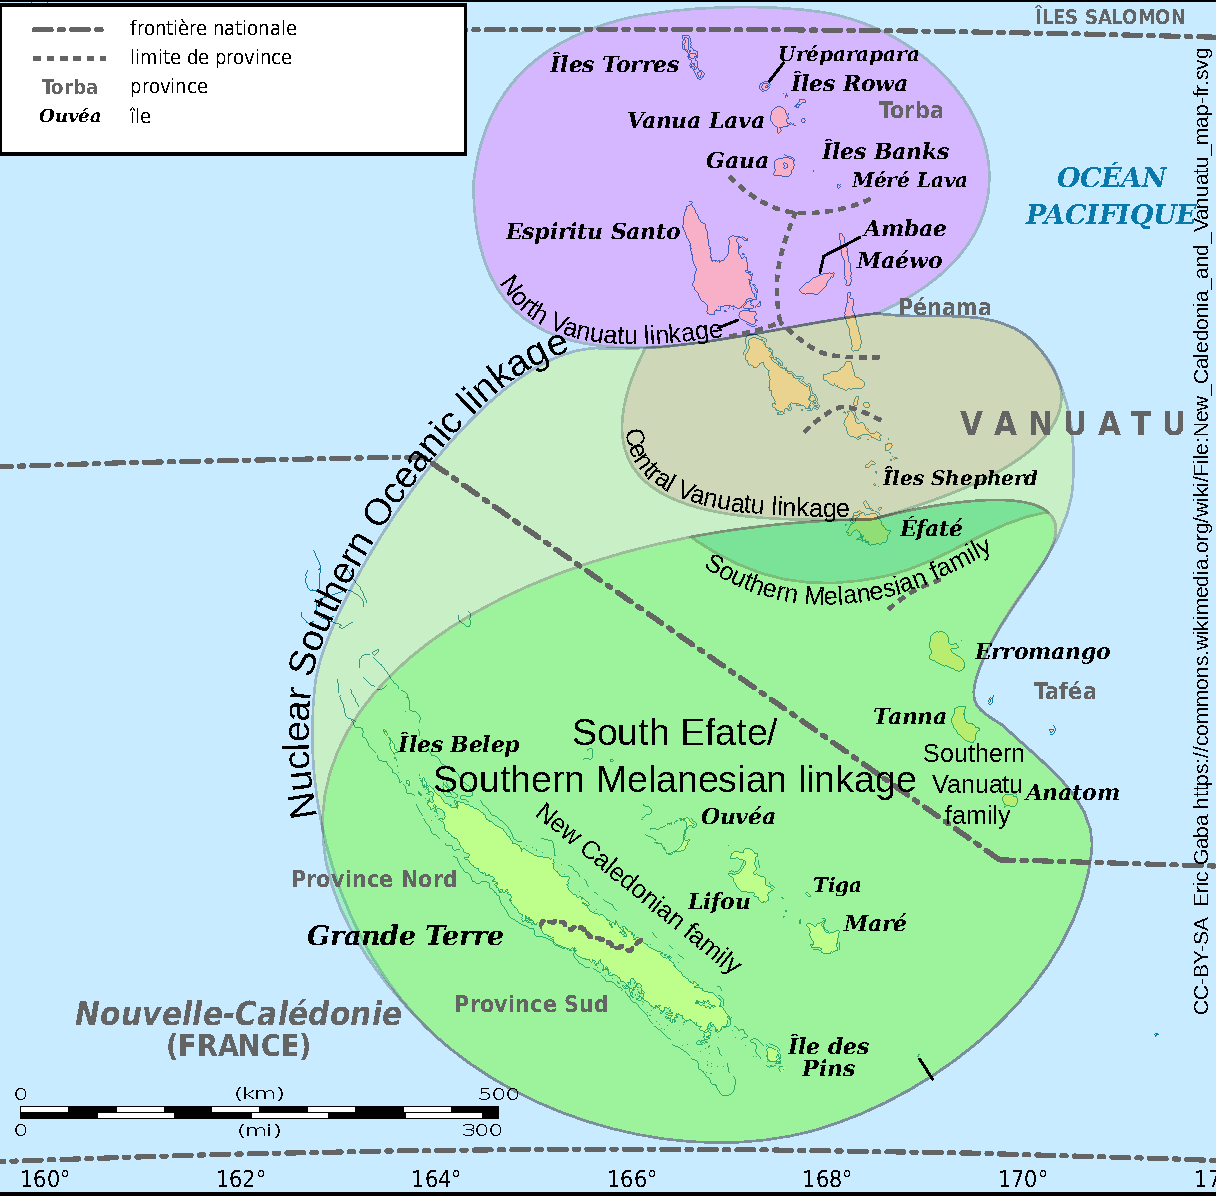
\includegraphics[width=\linewidth]{figures/lynchetal2022b.pdf}
	\caption{New Caledonian within the Southern Oceanic linkage \parencite[113]{lynch_oceanic_2002}}
	\label{fig:SouthOceanic}
\end{figure}
%\begin{table}
%	\caption{Proto-Oceanic consonantal phonemes, reproduced from \textcite[25]{ozanne-rivierre_phonologie_1982}}
%	\begin{tabular}{lccccccc}
%		& ``Labio-velar" &	Labial&	Dental&	Retroflex&	Palatal&	Velar&	Uvular\\
%		\multirow{3}{2cm}{Oral}&	&	*p&	*t&	*d&	*s/*ɟ&&\\
%		&&&&&&*k&*q\\
%		& *w&&*l&&*j&*R [ɣ]&	\\
%		Semi-nasal&	*ŋp/mp&	*mp&	*nt			&&*ns&*nk&\\	
%		Nasal&	*ŋm/m	&*m	&*n	&&	*ɲ&	*ŋ&	\\
%	\end{tabular}
%	\label{tab:POC_phon}
%\end{table}

Lynch uses the term ``Southern Oceanic" to refer to \qu*{a linkage whose members today comprise the 130 or so non-Polynesian languages of Vanuatu and New Caledonia} \parencites{lynch_southern_1999}[313]{lynch_efate-erromango_2004}. The linkage is defined by the innovations from Proto-Oceanic (POc) listed below, among others. 
\begin{itemize}
\item POc *R was dropped in absolute word-final position \parencite[313]{lynch_efate-erromango_2004} %, and t nonfinally in at least eight particular lexical items, though it was retained in most other etyma in nonfinal position." 
While northern New Caledonian languages do not feature \textit{-l} or \textit{-r} in non-loans, possessed forms hint at a merger with \textit{-t} rather than an apocope; compare Vamale \textit{fedat} \qu{blood} from POc *daaR to its possessed form \mbox{\textit{fedala-}.}
%[\ldots] A number of forms containing a bilabial in an earlier protolanguage replaced this with a labiovelar in PSO (see Lynch 2002). 
\item ``Third person pronouns accreted *na-." \parencite[313]{lynch_efate-erromango_2004} The singular article *na- was not conserved in New Caledonian, but \textcite[197--201]{ozanne-rivierre_proto-oceanic_1992} argues that a trace was responsible for some non-etymological prenasalized consonants \parencite[316]{lynch_efate-erromango_2004}. Compare *talik \qu{sea} $\rightarrow$ Vamale \textit{ⁿjati}. 
\item ``POc *k $\rightarrow$ Proto-Southern Oceanic (PSO) *g in some pronouns" \parencite[316]{lynch_efate-erromango_2004}. Compare \begin{itemize}
\item *POc *kita \qu{1\gl{pl}.\gl{incl}} $\rightarrow$ Southern Melanesian *gida or *gadV $\rightarrow$ Vam. \textit{gase}
\item  *POc *ko \qu{2\gl{sg}} $\rightarrow$ PNC, and Vam. \textit{go}
\item *POc *ka[m]u, *kamiu \qu{2\gl{nsg}} $\rightarrow$ PNC *ga(m)u $\rightarrow$ Vam. \textit{gau} \qu{2\gl{du}}
\end{itemize}
\item ``The ancestral system of two transitive suffixes reduced to one (or none)." \parencite[313]{lynch_efate-erromango_2004}. This relates to the transitive suffixes *-akini and *-i, both of which may still have reflexes in Vamale in the form of \textit{-ke} and \textit{-i}, respectively (see \sectref{ssec:ke_i}). While \textit{-i} is found in many northern languages, \textit{-ke} may now be unique to Voh-Koné. This potential disagreement with Lynch is grounds for more research.
%* A locative preposition PSO *(a,i)lo developed from the POc noun *lalo- 'inside'. 
%* POc *mataqu 'right (hand/side)' underwent metathesis as PSO *matuqa (see 2.3.4 below). There are some irregular developments in other lexical items, as well as some apparent lexical innovations." 
\end{itemize}
\largerpage

Southern Oceanic contains the Southern Melanesian family, defined amongst other things by its voicing of the initial plosive in certain pronouns (e.g. POc *kita \qu{1\gl{incl}} $\rightarrow$ SM *gida, later *gadV $\rightarrow$ Vam. \textit{gase}\slash\textit{gasu}) \parencite[317]{lynch_efate-erromango_2004}. New Caledonian as a family is well-defined by sound changes, listed below, and some lexical innovations \parencite[316]{lynch_efate-erromango_2004}. \Cref{tab:PNC-VK} summarizes and illustrates some of the consonant sound changes from Proto-Oceanic through Proto-New Caledonian, to modern-day Vamale and Bwatoo.

\begin{itemize}
	\item Merger of POc *c, *s $\rightarrow$ *s
	\item Merger of POc *n, *ñ, *l $\rightarrow$ *n
	\item Loss of POc *R and *y
	\item POc *puV  $\rightarrow$ PNC *pʷV
	\item POc *ai $\rightarrow$ PNC *e\slash *eː \parencite[317]{lynch_efate-erromango_2004}
\end{itemize}
\vskip-\baselineskip
\largerpage[2.5]
\begin{longtable}{llll}
	\caption{Voh-Koné reflexes of POc forms\label{tab:PNC-VK}}\\
	\lsptoprule
	\multicolumn{2}{l}{POc form} &  Bwatoo & Vamale\\\midrule\endfirsthead
	\midrule
	\multicolumn{2}{l}{POc form} &  Bwatoo & Vamale\\\midrule\endhead
	\endfoot\lspbottomrule\endlastfoot
	\multicolumn{2}{l}{Proto-Oceanic} & \\
	& *p &&\\
	\multicolumn{2}{l}{PNC} & \\
	& *p, *pw $\rightarrow$ v, vʷ	&&\\
	& *paRi \qu{ray(fish)}&\textit{ve}& \textit{ve}\\
	%	*pulu	\qu{hair}&	\textit{vuu}-	&	\textit{vuu}-\\
	& *poñu	\qu{turtle}&	\textit{vʷen}	&	\textit{vʷen}\\
	\multicolumn{2}{l}{PNC} & \\
	& *pp, *ppw	$\rightarrow$ f, fʷ&&			\\
	& *posi	\qu{press}&	\textit{fʷati}	&	\textit{fʷati}\\
	\multicolumn{2}{l}{POc} & \\
    & *d / *r&&\\
	\multicolumn{2}{l}{PNC} & \\
    & *t, *nd $\rightarrow$ ⁿd&&\\			
	& *daun	\qu{leaf}&	\textit{ⁿdoon}	&	\textit{ⁿdoon}\\
	& *daRoq	\qu{ground}&	\textit{ⁿdoot}	&	\textit{ⁿdoop}\\
	\multicolumn{2}{l}{Proto-North} & \\
	& *tʰ&&		\\
	& tʰat	\qu{pandanus}&	\textit{tʰat}&		\textit{tʰat}\\
	& tʰap	\qu{oral thrush}&	\textit{tʰap}&	\textit{tʰap}	\\
	%tʰoo	&	& tʰoo	&&	\\
	\midrule
	\multicolumn{2}{l}{POc} & \\
	& *t&&\\
	\multicolumn{2}{l}{PNC} & \\
	& *t̪, *d̪ $\rightarrow$ ⁿɟ&&\\
	& *tasi	\qu{younger sibling}&\textit{ⁿɟati}- &	\textit{ⁿɟati}-\\
	%& (same gender)&&&\\
	& *tupa	\qu{grandfather}&\textit{ⁿɟiᵐbu}-ⁿɟiᵐbu-\\
	\multicolumn{2}{l}{PNC} &\\
	 & *tt $\rightarrow$ θ/s&&\\			
	%	*tuka	\qu{elder}&	\textit{θia}-& \textit{sia}\\
	& *tumpuq	 \qu{swollen}&\textit{θiᵐbu} &	\textit{siᵐbu}\\
	\midrule
	\multicolumn{2}{l}{POc} & \\
	& *s&&\\
	\multicolumn{2}{l}{PNC} & \\
	& *s, *ⁿs $\rightarrow$ d/t&&\\
	%*sai&	who?	& ⁿde&	kai\\
	& *sapa	\qu{what?}&	\textit{ⁿda}&	\textit{ⁿda}\\
	& *sake	\qu{go up}	& \textit{ta}	&	\textit{ta}\\
	& *suRi	\qu{bone}&	\textit{ⁿduu}-	&	\textit{ⁿduu}-\\
	\multicolumn{2}{l}{PNC} & \\
    & *ss $\rightarrow$ tʰ&&			\\
	& *susu	\qu{breast}&	\textit{tʰi}	&	\textit{tʰi}\\
	& *suki	\qu{pierce} &	\textit{tʰi}&		\textit{tʰi}\\ % <<<--- Enlarge 2nd Table Page.
	\midrule
	\multicolumn{2}{l}{POc} & \\
	 & *k&&\\
	\multicolumn{2}{l}{PNC} & \\
	& *k $\rightarrow$ ð/j \goodtilde ∅ &&\\			
	& *kulit	\qu{skin}&\textit{ðii}&\textit{i-}\\
	%*kuluR&&&&\\
	%	*kutu	\qu{lie (parasite)}&	\textit{ði}&\textit{i}\\
	& *kuRita \qu{squid}&\textit{ðiia}&\textit{iᵐbwen}\\
	\multicolumn{2}{l}{PNC} & \\
	& *kk $\rightarrow$ θ/s&&\\			
	& *kuku	\qu{claw}&	\textit{θi}-	&	\textit{si}-\\
	& *kau	\qu{swim}&	\textit{θoom}&		\textit{soom}\\
	\midrule
	\multicolumn{2}{l}{POc} & \\
	 & *q &&\\
	\multicolumn{2}{l}{PNC} & \\
	& *q $\rightarrow$ ɣ/∅&&\\
	& *qusan	\qu{rain}&\textit{ɣuta/ wuta}& \textit{uta}\\
	& *qupi	\qu{yam}&\textit{ɣuu}	&	\textit{uvu}\\
	& *qata	\qu{man} &\textit{ɣau}&\textit{ɣaju}\\
	& *qaso	\qu{sun}	& \textit{ɣat}&	\textit{ɣat}\\
	\multicolumn{2}{l}{PNC} & \\
	& *qq $\rightarrow$ x&&\\				
	& *quma	\qu{grow, cultivate} &\textit{xuum}&\textit{xumi}	\\
	& *qulos	\qu{worm}& \textit{xun̥at}&\textit{xun̥at}\\
\end{longtable}


\begin{sloppypar}
The Southern Oceanic languages spoken in New Caledonia can be split roughly into two groups: Mainland (i.e. \textit{Grande Terre}) languages, and the three Loyalty Islands languages Iaai, Drehu, and Nengone \parencite{ozanne-rivierre_proto-oceanic_1992}. Mainland languages split into northern and southern languages (see \Cref{fig:Mainland}), with a tendency for northern languages to have 5 or so vowel phonemes and over 35 consonant ones, and an opposite trend for large vowel inventories and small consonant ones in the South \parencite[25]{ozanne-rivierre_phonologie_1982}. In the North, a Far Northern branch (\textit{Extrême Nord} in French) and a Northern branch split into some dozen languages (see \Cref{map:North} for a map). 
\end{sloppypar}\largerpage


\begin{figure}[H]
 		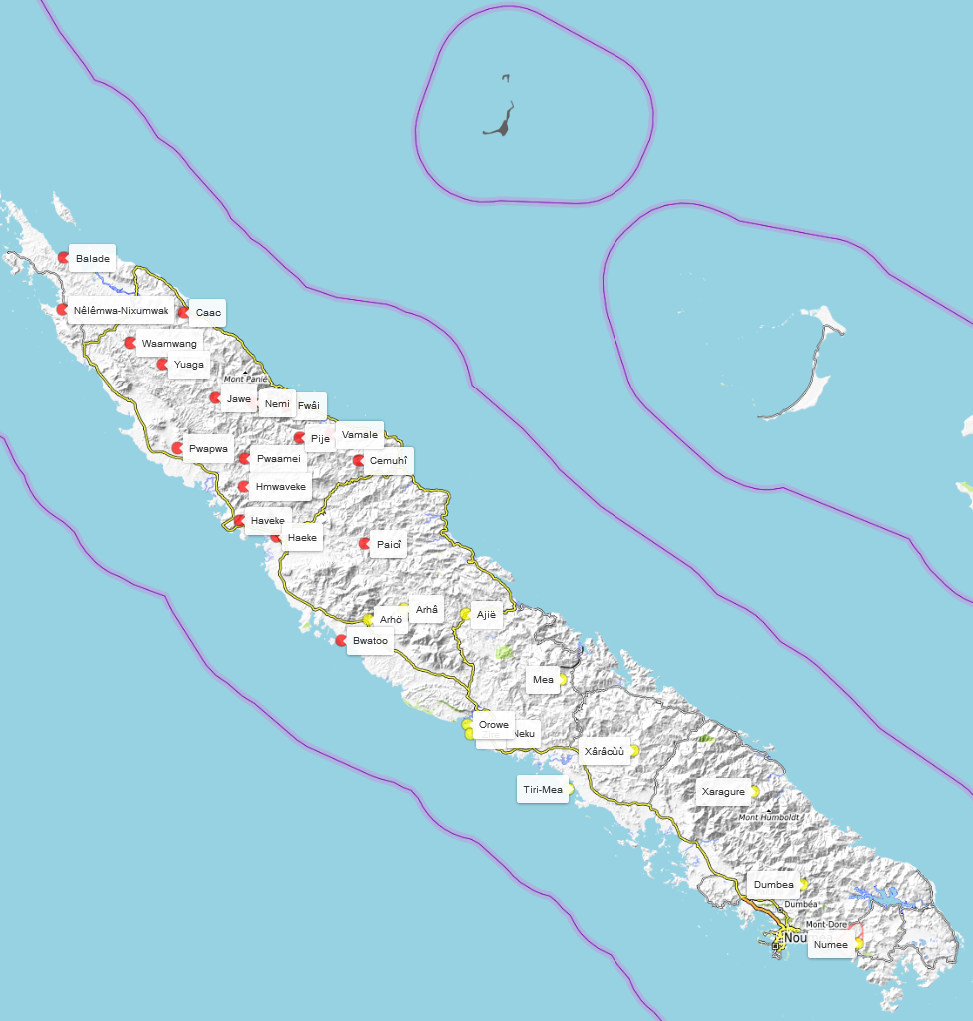
\includegraphics[width=\linewidth]{figures/Mainland_New_Caledonian}
		\caption{Mainland New Caledonian, North (red) and South (yellow) \parencite{hammarstrom_mainland_2020}}
 		\label{fig:Mainland}
\end{figure}


 %The Northern subgroup splits into three groups on the grounds of shared innovations: the small Extreme North group, the tonal Center group, and the North one, the latter of which includes Vamale's linkage Voh-Koné.
 The latter is split into the so-called Hienghène cluster, the Voh-Koné dialects, and the tonal languages Cèmuhî and Paicî, to which Voh-Koné is more closely related than to the other branches, \parencite[19]{rivierre_bwatoo_2006} see \Cref{fig:NorthTree} for a language tree. The language described in this book is part of the Voh-Koné cluster. The question of dialect vs language, as well as of the name given to the variety in question, will be addressed in \sectref{sec:LanguageName}.  

Voh-Koné is defined as a group mostly by phonological changes that set it apart from the rest of the Northern and Far Northern languages. Comparing sound changes in the Northern family is difficult due to sparse data. Valuable work was done by Haudricourt \parencite[73--97]{haudricourt_langues_1948} and especially Ozanne-Rivierre (\citeyear{ozanne-rivierre_structural_1995}, \citeyear{ozanne-rivierre_proto-oceanic_1992}). The following is mostly a summary of her work, with some Vamale data added. 

Compared to other Northern languages, Voh-Koné is mostly distinct by its lenition of *c $\rightarrow$ j and initial *p to v (see \Cref{fig:NorthTree}). The latter was dropped in some Vamale words such as the singular article *\textit{vi} $\rightarrow$ \textit{i} (but not the language's name). %Furthermore, Voh-Koné palatalized \textit{*t-} to /c/, a sound change the group shares with Jawe.
Geminates of *q, *k, *p, historically the result of reducing the first syllable in reduplicated contexts, yielded aspirated initial consonants everywhere in the North \parencite[57]{ozanne-rivierre_proto-oceanic_1992}, but have voiceless fricative reflexes in Voh-Koné (see \Cref{tab:PNC-VK}). Voh-Koné languages do have aspirated plosives which evolved from the same source, too, however. This is partly due to borrowing, but given their almost exclusive occurrence before nasal vowels, this study suggests that the leniting sound changes which led to a fricativization did not occur completely (see \sectref{ssec:Aspiration}).\largerpage


\begin{figure}[H]
	\begin{forest}
		for tree={
			forked edges,
			child anchor=west,
		    parent anchor=east,
		    grow=east,
		    anchor=west,
			align=center,
			inner sep=0pt,
		}[~
		[Extreme North]
		[Other Northern\\Languages
		[Nemi-Pije-Fwâi-Pwaamei-Pwapwâ \\{*mbw, mb ({/}\_o, u) $\rightarrow$ ŋgw}\\{*}mw $\rightarrow$ ŋgw
		[Nemi-Pije-Fwâi \\{*t $\rightarrow$ t, c ({/}\_i, e)}]
		[Pwaamei\\{*}t $\rightarrow$ c\\{*}c $\rightarrow$ y]
		[Pwapwâ\\{*}t $\rightarrow$ c]
		]
		[Jawe \\{*}t $\rightarrow$ c]
		[Voh-Koné-Cèmuhî-Paicî\\{*}c $\rightarrow$ y \\{*}t $\rightarrow$ c
		[Voh-Koné \\{*}p $\rightarrow$ v]
		[Cèmuhî-Paicî\\{*}CʰV $\rightarrow$ CV́]
		]
		]
		]
	\end{forest}
	\caption{Language tree of some North New Caledonian languages \parencite[63]{ozanne-rivierre_structural_1995}}
	\label{fig:NorthTree}
\end{figure}


 %  Another view, based on sound changes, places the Center group within the Northern languages, as represented in \Cref{fig:NorthTree} (\todo{whose view?}).%\begin{figure}
\begin{forest}
for tree={
%fit=band,
    child anchor=west,
    parent anchor=east,
    grow=east,
    draw,
    anchor=west,
  align=center,inner sep=0pt,
  {},
  }
[Northern 
  [
	[Extreme North
  [Caac]
  [Nêlêmwa-Nixumwak
  [Nêlêmwa]
  [Nixumwak]
  ]
  	]
  [Nyelayu]
  [Yuanga]
  ]
  [North (Proper)
	[Hienghène Languages
		[Nemi-Pije-Fwâi]
		[Pwaamei]
		[Pwapwâ]
	]
		[Jawe]
		[Voh-Koné-Cèmuhî-Paicî
			[Voh-Koné
				[Vamale]
					[Usa]
				[Hmwaveke]
				[Haveke]
				[Haeke]
				[Bwatoo]
			]
			[Cèmuhî-Paicî]
		]
	]
]
\end{forest}
\label{fig:NorthTree}
\caption{Language Tree of the North New Caledonian languages (\cite{ozanne-rivierre_structural_1995}:63 and )}
\end{figure}

Vamale is a member of the Voh-Koné languages, a group of mutually mostly intelligible varieties which forms a belt on the western shore from Voh to Népou including Koné and Baco, then follows the Tiéta river upstream and breaks off around Temala, before picking up again in the east around Tiendanite, Ouen Kout and We Hava (see \Cref{map:North}). As is typical of dialect chains, the varieties furthest apart have distinct grammatical morphemes, distinct lexicon, and different phonological systems. Because of this, Vamale and Bwatoo are not readily understood by speakers of the other variety. \Cref{tab:LeenhardtPN} compares Voh-Koné pronouns, along with Pwapwâ, a neighbor of Bwatoo, as they were recorded in the 1940s.  %The Voh-Koné languages form the Northern group of New Caledonian with the Hienghène languages, Pwapwâ, and Pwaamei, and the Central subgroup of tonal Cèmuhî and Paicî,  See \Cref{fig:NorthTree} for an illustration.
 
\begin{figure}
	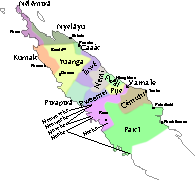
\includegraphics[width=\linewidth]{figures/north_new_caledonia2.pdf}
	\caption{Northern New Caledonian languages \parencite[45]{ozanne-rivierre_structural_1995}}
	\label{map:North}
\end{figure}

\begin{sidewaystable}
	\caption{Voh-Koné object-indexing pronouns after \textcite[504--507]{leenhardt_langues_1946}, modern Vamale added on the left.}
	\begin{tabular}{lllllllll}%{p{1.6cm}|p{1cm} p{1cm}lllll|l}
	\lsptoprule
		& \multicolumn{2}{c}{Vamale}&	Hmwaveke&	Waamwang&Haveke&	Haeke&	Bwatoo &Pwapwâ\\\cmidrule(lr){2-3}
		&   now   & 1946 & \\\midrule
		1\textsc{sg}	&\textit{ (e)o}&	\textit{o}&	\textit{yo}&	\textit{ng}&	\textit{ng}&	\textit{ong/ ng}&	\textit{ng}&\textit{ng}\\
		2\textsc{sg}&	\textit{ko}&	\textit{ko}&	\textit{go}&	\textit{m}&	\textit{go}&	\textit{go/ m}&	\textit{m}&\textit{m}\\
		3\textsc{sg}&\textit{(e)a}&	\textit{kon, ke}\footnote{Note that \textit{kon} may refer to an oblique marker \textit{ko-n} and \textit{-ke} is a transitive suffix.}&	\textit{kon, ke}&	\textit{n}&	\textit{gon}&	\textit{mon/ n}&	\textit{n}&\textit{n}\\
		1\textsc{du}.\textsc{incl}&	\textit{ju}&	&&&	&&					\textit{ju}&\\
		1\textsc{du}.\textsc{excl}&	\textit{bu}&			&&&&&				\textit{bu}&\\
		2\textsc{du}&	\textit{u}	&			&&&&&			\textit{u}&\\
		3\textsc{du}&	\textit{lu}	&					&&&&&	\textit{lu}&\\
		1\textsc{pl}.\textsc{incl}&	\textit{ga}&	\textit{ga}&	\textit{ga}&	\textit{je?}&	\textit{gaie}&	\textit{ngaie/ je}&	\textit{je}&\textit{je}\\
		1\textsc{pl}.\textsc{excl}&	\textit{be}&	\textit{be}&	\textit{be}&	\textit{be}&	\textit{gabe}&	\textit{ngabe/ be}&	\textit{be}&\textit{be}\\
		2\textsc{pl}&	\textit{gavʷe}&	\textit{gae}&	\textit{vʷe}&	\textit{we}&		\textit{gae}& \textit{o}&	\textit{e}&\textit{e}\\
		3\textsc{pl}&	\textit{le}&	\textit{le}, \textit{ke}&	\textit{le}&	\textit{le}&	\textit{le, ke}&	\textit{le, ke/ le}&	\textit{le}&\textit{le}\\
	\lspbottomrule
	\end{tabular}
	\label{tab:LeenhardtPN}
\end{sidewaystable}
%The possible closer relationship between Jawe and Voh-Koné languages has not yet been studied in detail, but may be of interest. Jawe, like Vamale and other Voh-Koné languages, has seen the (typologically unremarkable) sound change *t $\rightarrow$ c, as have the Hienghène languages. However, Pije and Nemi have conserved the old post-nasalised consonants k\textsuperscript{n}, t\textsuperscript{n}, which in Jawe and Voh-Koné gives k\textsuperscript{h}Ṽ, k\textsuperscript{h}Ṽ, with the postnasalisation expressed on the vowel (eg. \textit{kniik} $\rightarrow$ \textit{khîî} \qu{swamp fowl}), see \Cref{ssec:Aspiration}. On the other hand, \Cref{map:languages_1917}, showing the situation in 1917, places a contiguous Nemi-speaking land between the Jawe and Vamale areas. Jawe may have simply evolved alongside Voh-Koné and Cèmuhî-Paicî before the current geographical situation was set.

The languages of Voh-Koné probably spread from the eponymous region on the west coast to the Upper Tiéta valley, where Hmwaeke\footnote{\textit{hmwaeke} is a common greeting in the eponymous variety meaning \qu{how [is it going]?}.} is spoken. Until the early 20\textsuperscript{th} century, the neighboring valleys of the Pamale and its tributaries were inhabited by some 2,000 people according to oral tradition \parencite[62]{couhia_pascal_2008}. Since this region fell under colonial control only in the wake of World War I, no census before the Tipije war can confirm or contest this number. The entire population of the valley was either killed or scattered (see \chapref{chap:Tipije}). A map of the main movements can be found in \Cref{map:fugitives}. Those who went west assimilated into their linguistic cousins, whereas the eastward fugitives kept a language alive which they call Vamale today. Leenhardt called it \qu{'Moaeke} of the East Coast and counted 50 speakers \parencite[162]{leenhardt_langues_1946}.

%the kon/ke thing might be xale koon, xaleke X?
%\todo{include? cuz looks like OBJ paradigm}

%\subsection{Phonological clues}

%POc *q $\rightarrow$ Proto-New Caledonian, changed to voiced fricatives in Voh-Koné, where other North New Caledonian languages kept \textit{k} \parencite[57]{ozanne-rivierre_structural_1995}. The geminate *qq became *kh in Proto-North, and a palatal \textit{c} in modern languages

%POc  developed stops \parencite[200]{ozanne-rivierre_proto-oceanic_1992}. 

%The POc tap consonant *d / *r as well as the fricative *s changed to plosives, e.g. *\textit{sake} $\rightarrow$ \textit{ta} \qu{go up} \parencite[19]{rivierre_bwatoo_2006}.
\begin{sloppypar}
Within Voh-Koné, the major division opposes western, coastal varieties and eastern, mountain-based ones.
Interdental fricatives /θ/ and /ð/ are features of Bwatoo, Haveke, Haeke and Waamwang, whereas Hmwaveke and Vamale present the alveolar fricative /s/ instead of /θ/, and have lenited /ð/ to /j/, or dropped it before /i/ (e.g. *kulit \qu{skin} $\rightarrow$ Bw. \textit{ðii}, Vam. \textit{i-}).
\end{sloppypar}

Proto-Oceanic initial *q has become /ɣ/ in Vamale, except before /u/ (e.g. *\textit{qusan} \qu{rain} $\rightarrow$ \textit{uta}); western varieties keep /ɣ/ before /u/. The only case of a voiced fricative before /u/ is an allophone of /h/.
[ɣ] is also dropped before /o/ (Bwatoo \textit{ɣop} \qu{high tide}, \textit{op} in Vamale).

Intervocalic /v/ within a morpheme is rare, which is a contrast to the western languages.\footnote{Except for \textit{fava} \qu{4}, but Pije \textit{hovac}, Fwâi \textit{fovec} \parencite[261]{haudricourt_dictionnaire_1982}. Bwatoo \textit{fae}, Oundjo-Haveke \textit{favac} \parencite[135]{rivierre_bwatoo_2006}.} Hmwaveke, part of the mountain group, still shows intervocalic /v/ lost in Vamale, which suggests that this sound change originated in the East. Finally, %most Voh-Koné languages kept /p/ in places where Vamale now has /v/ (e.g. \textit{vamale}), and 
some final consonants (chiefly /k/ and /c/) were lost in Vamale that remain in Hmwaveke.

Historical sources suggest %In conclusion, there are western, coastal varieties which probably form 
a sort of \textit{Urheimat}, given that Guiart mentions a bigger Haekic coalition on the west coast before the Paicî influx of the 18th and 19th centuries \parencite[131,260]{guiart_chefferie_1963}. Compare the map by Leenhardt in \Cref{map:languages_1917} to \Cref{map:North}: Voh-Koné languages retreated to the North, and the coast between Koné and Poya is almost exclusively Paicî-speaking today. Interestingly, the map treats Pwapwâ and Pwaamei as dialects of Nemi. As the map, along with many of the language materials in the book was compiled using second-hand accounts \parencite[xi,xiii,xlviii]{leenhardt_langues_1946}, its accuracy depends on the area depicted. Since Leenhardt himself traveled to Pamalé in 1903 \parencite{leenhardt_figures_1978}, we can rely on the map for Vamale's historical position, even if it was inaccurate by the time of its publication. Until 1917, Vamale was spoken in an area inhabited since 420–610 AD \parencite[172]{sand_certainly_2012} (though probably not by Voh-Koné speaking people), and represents the easternmost point of a putative inward expansion of a dialect continuum. 

Spatial proximity %close contact of the languages 
groups coastal Haveke and mountainous Hmwaveke together, so that there is a middle zone, as is typical of dialect chains. In addition to this blurring factor, language contact changed dramatically in the last century, with an influx of refugee Hmwaeke and Vamale speakers that changed Haveke and Hmwaveke. Vamale itself may have changed faster in its relative isolation.

\begin{figure}
	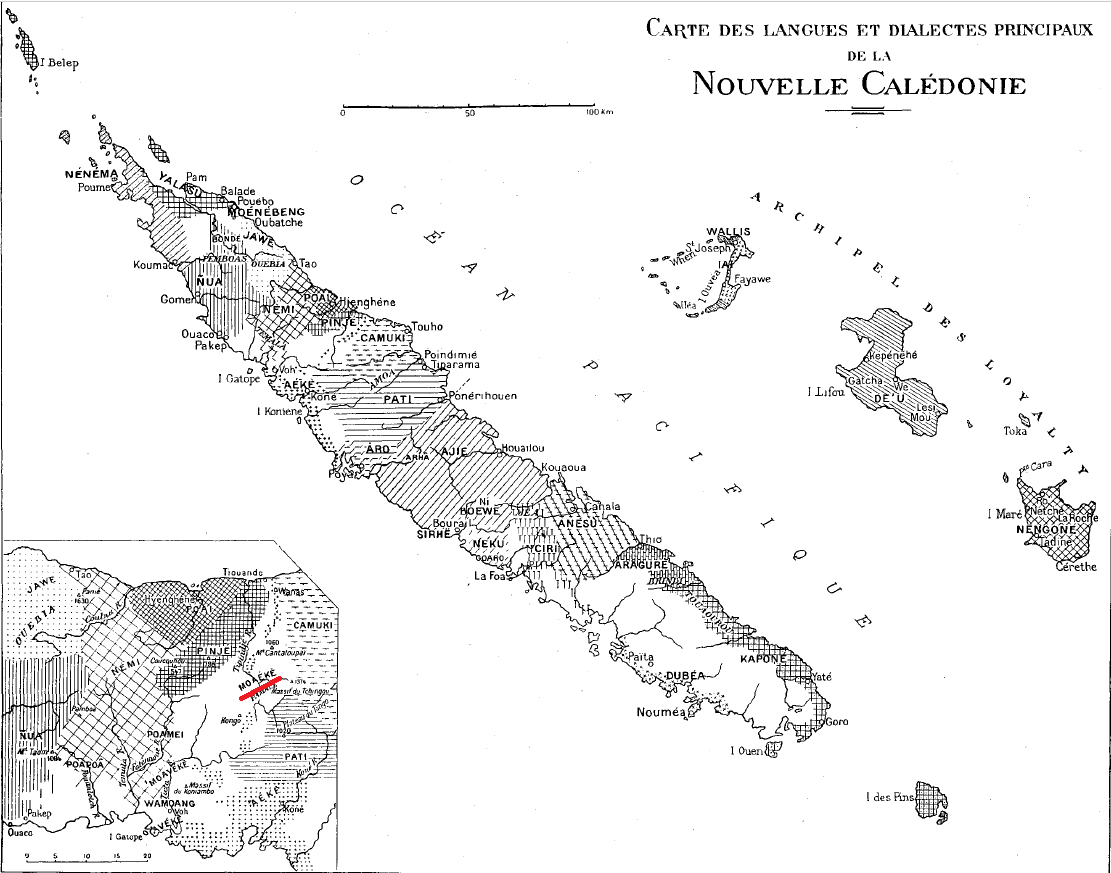
\includegraphics[width=\linewidth]{figures/leenhardt_map658}
	\caption{Languages in the region around 1917 \parencite[658]{leenhardt_langues_1946}, with Vamale (``Moaéké") underlined in red.}
	\label{map:languages_1917}
\end{figure}
%\begin{table}
%	\caption{Some isoglosses within Voh-Koné}
%	\begin{tabular}{cccccc}
%								& Vamale&					Hmwaveke&	Haveke&	Haeke&Bwatoo\\
%		\hline&&&&&\\
%		Intervocalic v&		No\footnotemark &	Yes &Yes& No&No\\
%		Initial ɣ-& No & No & Yes & Yes & Yes\\
%		Interdental fricatives & No & No & Yes & Yes & Yes\\
%		-p&						Yes& 							Yes&Yes	&Yes&-t\\
%	\end{tabular}
%	\label{tab:VK_inner}
%\end{table}
%\footnotetext{Except for \textit{fava} \qu{4}, but Pije \textit{hovac}, Fwâi \textit{fovec} \parencite[261]{haudricourt_dictionnaire_1982}. Bwatoo \textit{fae}, Oundjo-Haveke \textit{favac} \parencite[135]{rivierre_bwatoo_2006}}
 
 \begin{figure}
	\fittable{%
 	\begin{forest}
		forked edges,
		for tree={align=center,grow=south}
		[Voh-Koné
		[Coast
		[Haake\\Bwatoo]
		[(Waamwang)]
		[Haeke]
		[Haveeke]
		]
		[Mountain
		[West
		[Hmwaveke]
		[Hmwaeke]]
		[East
		[Usa]
		[Vamale]
		]]
		]
	\end{forest}}
 	\caption{Possible language tree of Voh-Koné languages}
 	\label{fig:VKTree}
 \end{figure}
 
 \subsection{Linguistic context}
 This section aims to describe how Vamale relates to other languages surrounding it.
 Historically, it is likely that the Voh-Koné languages spread eastwards into the mountains, which would suggest that Vamale/Hmwaeke is most closely related to Hmwaeke proper, then Hmwaveke, maybe Waamwang, and finally Haveke, Haeke, and Bwatoo.
 
 \is{Language contact}
 People formerly would cross the mountains on foot- and horse trails, leading to Pije, Fwâi, and Cèmuhî speaking areas, but more importantly other Voh-Koné speaking areas: Tiéta (Haveke), Temala (Hmwaveke), and some isolated houses in the middle, as well as diasporically in Bopope and Atéou. Nowadays, work in the nickel mines and the cargo ports, coupled with a lack of legal restrictions to buy cars without a driver's license, %and occasionally growing and selling cannabis 
 have afforded most families with the means of traveling long distances to visit relatives and maintain social ties. This, however, has also changed the languages with which Vamale speakers are in contact. Nowadays, cars dominate mobility and define it. Roads lead to Hienghène and Touho, so Fwâi and Cèmuhî have gained influence. Crossing the mountains leads through Cèmuhî and Paicî areas, and going to Tiéta and Temala takes up to 4 hours. %This means that the Vamale is in even more intense contact with the Hienghène languages and tonal Cèmuhî. 
 The nearest road connecting the coasts leaves the shore for the mountains at Touho, 30 km from the southernmost Vamale community, Téganpaïk. Tiéta,\footnote{Ceta/Caa-ta \qu{setting down the foot to go up, doorsill}} where Vamale's closest linguistic neighbor Hmwaveke is spoken, can only be reached via Voh (a journey of 3 hours minimum by car). As Rivierre notes, this has led to a differentiation of the former language Hmwaeke into Fa Tiéta (Hmwaeke mixed with Hmwaveke) and Vamale (influenced by Pije, Fwâi, and Cèmuhî)  \parencite[14]{rivierre_bwatoo_2006}. %The communities on the coast do not consider themselves to speak the same language as the Tiéta people, but call all Voh-Koné languages, including their own, by the same name: Vamale. 
 Furthermore, traveling used to imply staying somewhere for a while, since it was impractical to walk for days only to stay for a short while. This tradition of longer stays used to cause intensive language contact, and is now in decline. While there are still people alive who used to travel regularly to the other side, and mixed marriages connecting the two coasts are not rare, there is a real break between the speech communities. %Horses and foot trails having all but fallen out of use, movement nowadays follows car roads. 
 The two coastal villages Téganpaïk and Tiouandé are right on the national main road which runs along most of the east coast, while the others, We Hava and Tiendanite, are between 20 and 45 minutes by car from this main axis. The latter experience less contact, and less attrition.
 %important because language contact
 
 \begin{figure}
%  	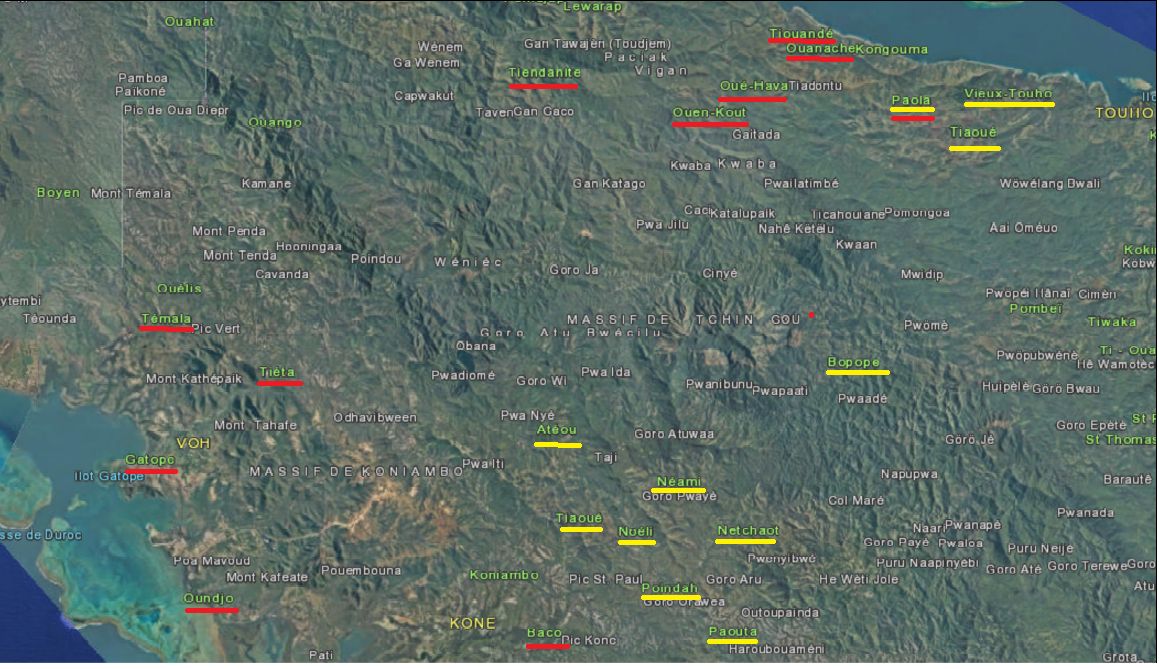
\includegraphics[width=\linewidth]{figures/map_languages.png}
 	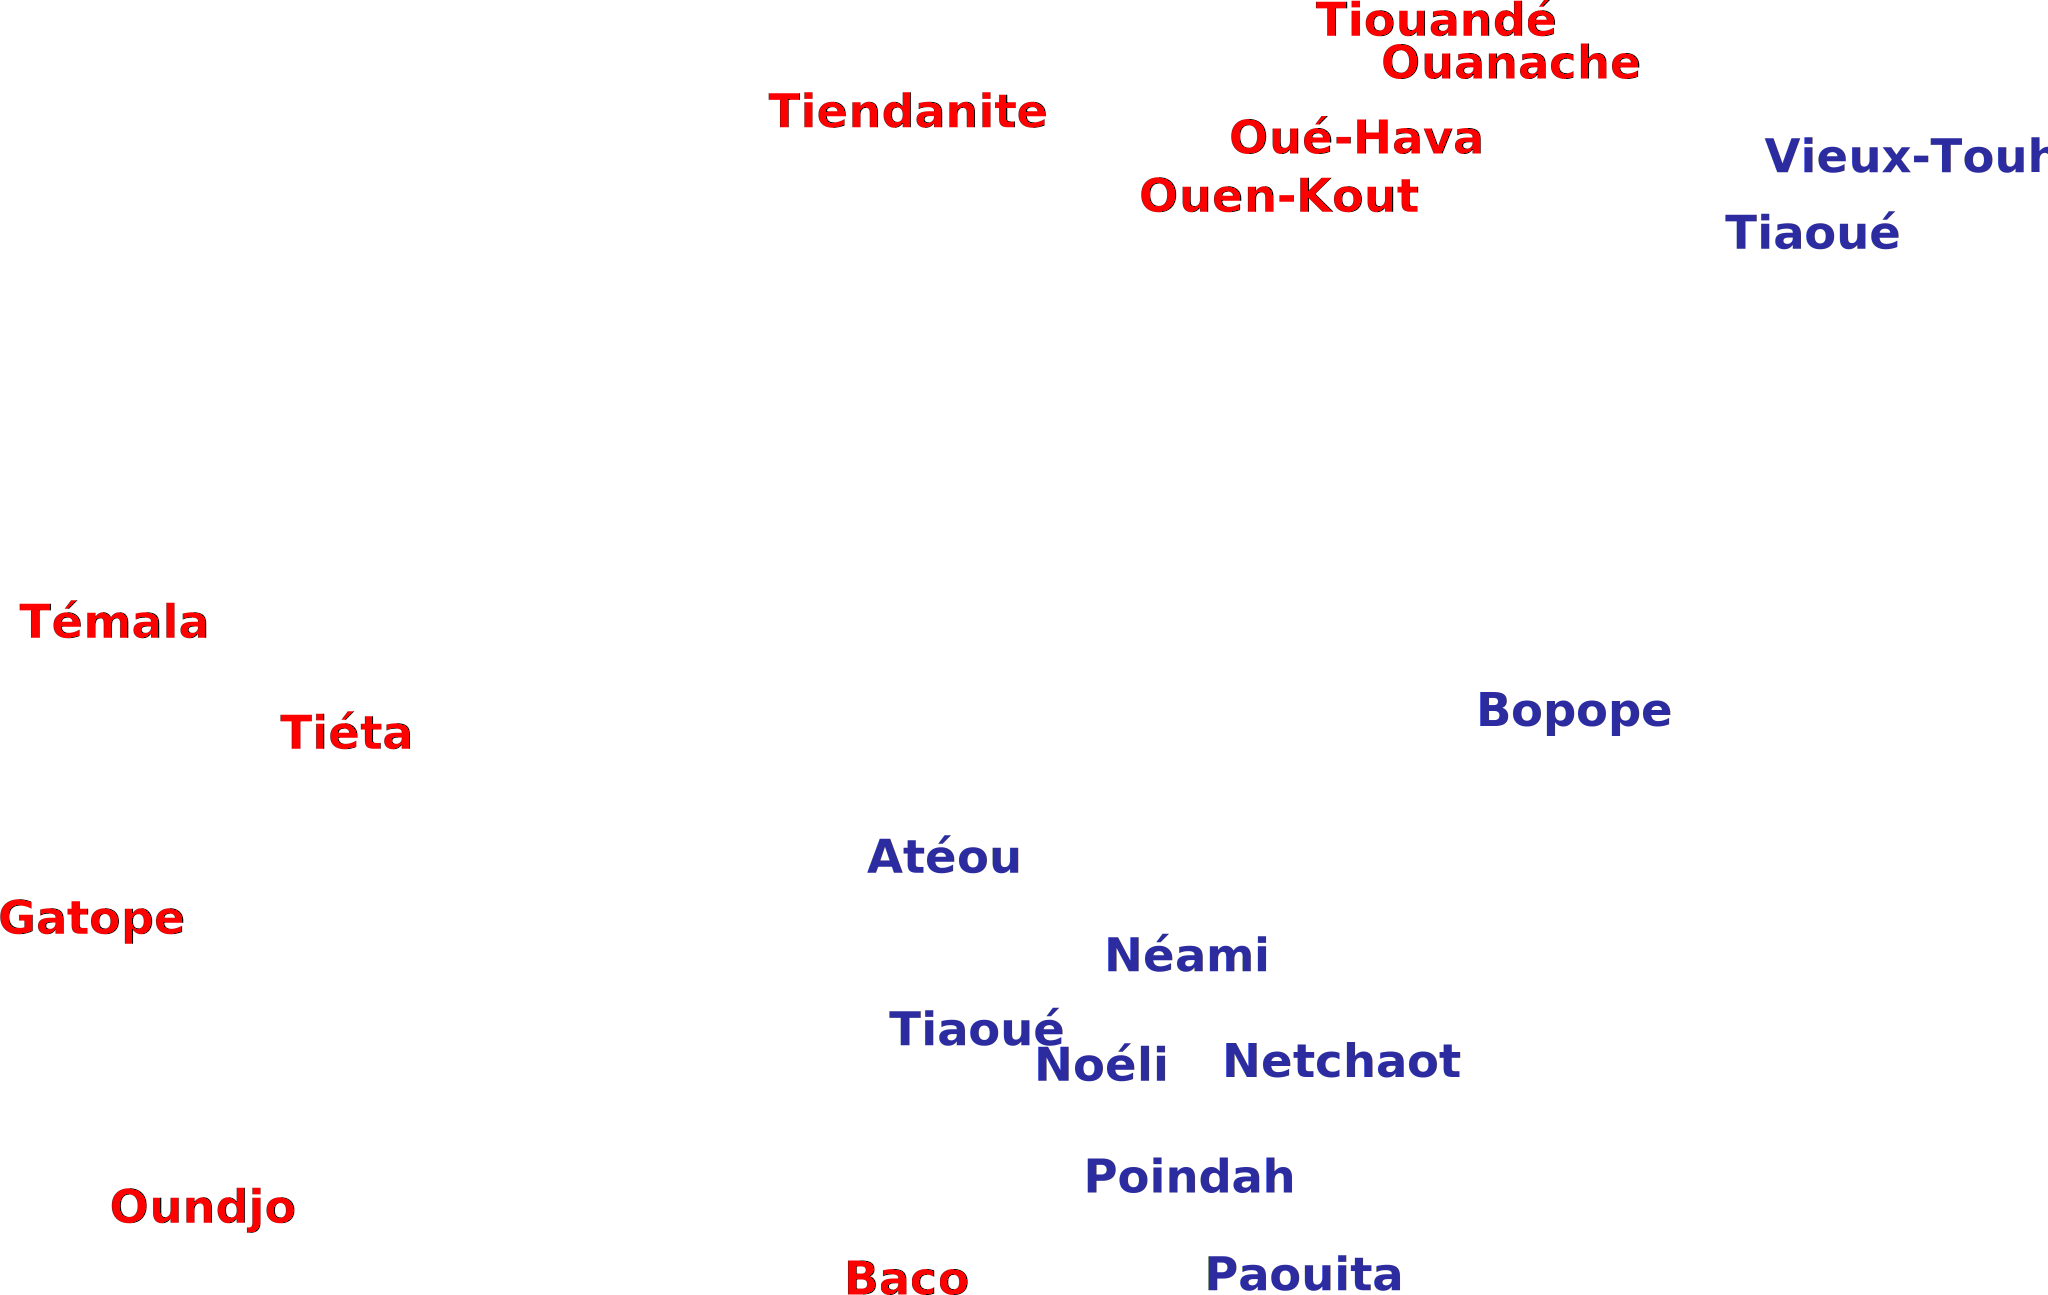
\includegraphics[width=\linewidth]{figures/vohkonepaicicemuhi.pdf}
 	\caption{Languages in the region, Voh-Koné-speaking villages in red, Paicî-Cemuhî-speaking ones in blue (adapted from \cite{gouvenementdelanouvelle-caledonie_explorateur_2019})\\\tiny © OpenStreetMap contributors. Tiles courtesy of Andy Allan}
 	\label{fig:map_languages}
 \end{figure}
 
 Vamale has been in contact with other, not readily intelligible, languages for centuries. %By providing a phonological description of the language, comparing the language to the rest of the cluster in depth will become possible. 
 It is surrounded by North Northern Caledonian languages of the Hienghène cluster, and Central Northern Cèmuhî, see \Cref{fig:map_languages}. While this is also the case for Haeke and Bwatoo (Haake), which mostly interact with Paicî, some Cèmuhî, and Pwaamei in the north, only Vamale is surrounded from all sides by non-Voh-Koné languages. Vamale has adopted the subject marker \textit{e=} \qu{1\gl{sg}}, as well as phonological traits from Cèmuhî (see \sectref{ssec:Vowel_Quality}), as well as loan phones from Pije. \citegen{leenhardt_langues_1946} description suggests that lexical changes have occurred. \parencite[162--168]{leenhardt_langues_1946}
 
 \begin{itemize}
 	\item \textit{da} \qu{who}, still used in western varieties, is now \textit{kai} \qu{who} in Vamale, and \textit{kaikai} \qu{for whom?} was substituted with \textit{nya(si/ko) kai}.
 	%\textit{xa} was a relativizer meaning \qu{X who does Y}, this is now \textit{a} like the unmarked one.
 	\item The indefinite articles have all changed: \textit{en} \qu{a, other}, still found as \textit{ven} in the Usa variety, is lost in Vamale, which now uses \textit{eca} \qu{\gl{indf}.\gl{sg}} and \textit{se} \qu{other}. \textit{men} \qu{\gl{indf}.\gl{pl}} and \textit{mun} \qu{\gl{indf}.\gl{du}} were used in demonstrative settings \parencite[165]{leenhardt_langues_1946}. Nowadays, putative equivalents would be \textit{ca} for the plural and \textit{muca} for the dual. 
 	\item There used to be more forms for adhortative exclamations (``vocative"), distinguishing adults from children (\textit{hai} and \textit{hnei}, respectively), whereas now there is only \textit{ha}.
 \end{itemize}
 
 \subsection{Multilingualism and variation}
 \label{sec:Multiling}
 \is{Code-switching}
 The author has met no-one between Téganpaik and Hienghène who speaks a Kanak language since birth without speaking another one. This is one of the first things someone will tell you: \qu*{I do Vamale a bit but also Pije and Fwâi}. People swear in three languages, they freely mix in words from other languages if they can't remember them, and they constantly code-switch functionally to mark their belonging to a group, to the description project, if they do not want somebody to understand, etc. This includes Usa, the variety spoken in Tiendanite. Speakers are able to adapt to coastal varieties, weave in Pije words, etc. In 2017, the author was present at the council of clans in Tiouandé, a monthly public meeting where all local affairs are discussed. I was there to give an update on the work. A conversation about a local criminal was done almost entirely in Pije, before the council switched back to Vamale. %Whether this was because Tiouandé is thought of as a Pije-speaking community, or because the criminal's clan is Pije-speaking, or, more likely, 
 This was likely due to privacy reasons, as they knew that I grasped some Vamale but no Pije. The choice of language among most middle age adults is functional and relatively free. There is thus probably no native speaker in the area who is not fluent or at least somewhat competent in another Kanak language. Male Cèmuhî speakers are an exception and usually only speak this one Kanak language; due to exogamy, many women come from another language area.
 
 \subsection{Neighboring languages}
 \label{ssec:neighbors}
 Vamale speakers have daily contact with other languages, most of which would not be readily intelligible. Pije is spoken in every Vamale-speaking village, and Cèmuhî by neighboring villages, as well as by local political authorities. Haeke, a Voh-Koné language, will also be discussed in some more detail below, not for its geographic proximity, but because the increased mobility of speakers has intensified contact with it. %An exception is Tiendanite-based Vamale Usa. It is very similar to Vamale, except for some archaisms, a different prosody, and some lexical differences.
 
 \subsubsection{Pije}
 \is{Pije}
 Pije (ISO 639-3 piz) is spoken in the same villages as Vamale. There is a coastal variety with about 70 speakers left; the Tipije varieties having all but disappeared due to the war. A mountain variety spoken in Tiendanite, called \textit{tha} \parencite[229]{haudricourt_langue_1968}, is relatively vital; it is the majority language there and practiced by many children (whereas Usa's youngest speaker is in her 20s). Pije is the most spoken indigenous second language of Vamale speakers. During elicitation sessions, Pije words were often given before being corrected. One reason for Pije's dominance in the area I'm focusing on is indigeneity: Pije is the land-owners' language here, the coast between Téganpaïk and Pedaa (Pindache) used to be in Pije-speaking hands, and a migration of Vamale speakers led to a complexification of the sociolinguistic situation. With the Vamale river flowing into the Tipije, language contact was always a fact of life in the upper valleys, but this contact has changed and intensified after the war. This also means that Pije is a language of prestige, the ``original" language, and many families reported a paternal (land-owning), Pije-speaking bloodline coupled to a maternal, Vamale-speaking one. Many residents were doubtful of the legitimacy of the project, as it should be Pije, more endangered and more autochthonous as it is, that should have been documented before Vamale. 
 
 \subsubsection{Fwâi}\is{Fwâi}
 Fwâi (ISO 639-3 fwa) is the language of Hye-hen (Hienghène, \qu{cry-walk}), the administrative center north of the Tipije river, and the school town of We Hava. The hospital, the market, an active cultural scene, and a bar, all attract residents of the three villages, and since the main road connecting Hienghène to the south runs through Tiouandé and Teganpaik, language contact is extensive. The main lexical influence seems to be swearwords, and the languages are not mutually intelligible.
 
 \subsubsection{Cèmuhî}\is{Cèmuhî}\largerpage
 Cèmuhi or Camuki (ISO 639-3 cam) is a tonal language with 3 register tones. It is spoken in the villages west of Téganpaïk up to Kokingone, and is the language of Great Chief Bouillant/Bwiyâ as well as most villages in the Great Chief's domain (to which most Vamale speakers belong). It is used for official purposes by the Great Chief's \textit{porte-parole} \qu{heralds}, and can thus be considered a regular contact language for Vamale, but is not intelligible with the latter and functional communication occurs in French. %The mayor of the commune's main town also speaks Cèmuhî, and uses it in poetry and stories he writes. 
 With around 3,300 speakers, it is one of the biggest languages in the area. 

 
 Vamale would have been surrounded by Cèmuhî speakers for some time before being moved to the coast. The villages Netchaot (Paicî\slash Cèmuhî) and Bopope (Cèmuhî), as well as the warring factions in the 1903 conflict Touho and Poyes, all spoke Cèmuhî. There was, however, a relatively stable and cohesive dialect chain of Voh-Koné languages from the west coast to Pamale, which suggests that for a while, contact happened eye-to-eye.
 
 \newpage
 \subsubsection{Haeke}\is{Haeke}
 \label{ssec:haeke}

 \begin{sloppypar}
 Haeke (ISO 639-3 aek) speakers, especially of the clans Wabealo and Cidopwaan, are tied through marriage to Vamale speakers, and according to Guiart, the mentioned clans claim to descend from the Paicî Naoutchoue/Naaucuwè lineage \parencite[92]{guiart_laire_1992}, with whom the Pei clan (important in Téganpaïk) is closely tied. Speakers of Vamale, thanks to cars, family ties (see the map \Cref{map:clans}) and frequent festivities, are now in more regular contact with other Voh-Koné varieties, especially Bwatoo and Haeke. However, the speakers the author spoke to were very aware of the differences between different speech practices and desirous to keep them distinct. Haeke is closer to Bwatoo and features typical Western Voh-Koné traits such as interdental fricatives, but as a funeral ceremony speech held in Haeke was understood by most Vamale speakers, some mutual intelligibility may be postulated. Haeke is highly endangered as well, and most contact happens in French. 
 \end{sloppypar}
 
 %\subsubsection{Conclusion}
 
 %Proud people, very motivated, but ridden with social problems and obstacles, hope that school will save the language, or other people.
 %That being said, the plural article \textit{ni} seems\begin{comment} to be a free variant of \textit{li}, and is used in all other Voh-Koné varieties.
 
 	%this is where we can maybe talk about their similarities and differences which has implications for what language is what language and what we consider the language we’re focusing on in this study and
 	
 	
 	
 	
 	%Other tips concerning politeness: avoid smelling food, always bring something (e.g. a package of rice) when invited to a meal, and know that the guest is supposed to eat first, then the men, then the women. If you stay for more than a day or two, offer to help with cooking and the dishes. Avoid touching the central post, leaning against a part of the house with a stretched-out arm, breaking a coconut indoors, and refusing anything offered multiple times, as this is as impolite as refusing any demand (for tobacco etc).
 	%
 	%Pei Dui's family, which comprises his woman from Maré, Élise and his daughter whom he had with a Paicî woman and who is in a boarding school in Poindimié, Elodie, moved from a small concrete house now cluttered with stuff, mostly papers, next to the concrete foundation (a concrete disk with a hole for the central post) of a torn down hut, to an empty house uphill of his adoptive mother's house and his adoptive brother Richard's house, who has a roofless hut next to it, the straw for which has been dry in his garden since 2013. Dui's new house was built with subsidies, the surrounding ground is rubble, Yaté the dog would guard it if she weren't so sweet. 
 	
 
 \section{Previous work}
 \label{sec:prev_work}
 \largerpage
 Vamale is almost exclusively an oral language. It is used in church (at least in Téganpaïk) for songs; Néa Galé of Baco has published some prose, and some songs are archived, recorded by Haudricourt in 1963 \parencite{nea_poesie_1963}. 
 The Protestant missionary and pastor Maurice Leenhardt was based in Houa\"ilou, but was active across the entire archipelago and wrote extensively about Kanak languages and cultures. His most important linguistic work is \textit{Langues et dialectes de l'Austro-Mélanesie}, published in 1946. Short grammar sketches on almost every language at the time are followed by a comparative word list of over 1,000 items. This is the most extensive work done on Vamale (``\textit{'Moaeke}") to this day. While a number of items were deemed by speakers to be loans from other languages, mostly Pije, the list is the only published trace of the names of gods, dances, and objects since lost.
 
André-Georges Haudricourt worked in New Caledonia between the 1940s and the late 1970s. The relevant articles are overviews over the phonological systems of all then-described languages (\citeyear{haudricourt_richesse_1961}), and grammatical typologies of the archipelago (e.g. \citeyear{haudricourt_langues_1948}, \citeyear{haudricourt_new_1972}, \citeyear{haudricourt_langues_1948}). Haudricourt's only work on Vamale, a dictionary project, was never published and is presumably lost \parencite[18]{rivierre_bwatoo_2006}. 

 %\todo{short descriptions}
 Jean-Claude Rivierre worked on Paicî (\citeyear{rivierre_dictionnaire_1983}) and Cèmuhî (\citeyear{rivierre_langue_1980}, \citeyear{rivierre_tonogenesis_1993}), as well as on Bwatoo (\citeyear{rivierre_bwatoo_2006}, a grammar sketch of 45 pages with a detailed dictionary following), and was the most important author on Vamale's immediate neighbors (e.g. \citeyear{rivierre_contact_1994}). He also assembled a precious dictionary of Hmwaveke containing Vamale items, unfortunately not yet published: \citetitle{rivierre_projet_}.\largerpage

%\subsubsection{Cannibalism}
%\is{Cannibalism}
%Cannibalism is a notorious part of traditional Kanak society. Although not directly relevant to the description or documentation of the language, the author believes it justified to say a few words about this stigmatizing and widespread connotation of the word ``Kanak". 
%Cook reports an aversion to cannibalism in Kanaks in 1774 \parencite[56]{sand_reconstructing_2000}. LaPérouse describes a cannibalistic population at constant war in 1788  \parencite[58]{sand_reconstructing_2000}. According to \citeauthor{bensa_political_1997}, a chief's power was based on the number of bodies controlled relative to neighbors. Following this, the destruction of enemies' bodies was one of the bases of chiefdom\is{Chiefdom} \parencite[89]{bensa_political_1997}. One reason for consuming the enemy is to avoid vengeance from the ghost of the departed. Destroying the corpse, according to \citeauthor{bensa_political_1997}, was seen as a way to prevent the deceased from becoming an ancestor, who counted as a body controlled by the deceased's clan, and would thus not have diminished the neighbor's power. But even this destruction does not seem to have been a total safeguard against revenge, since eating enemies happened outside of inhabited areas, to prevent villages from being haunted \parencite[96]{bensa_political_1997}, and \textit{nyawan xhwi} \qu{ghost of an eaten person} plays a role in folklore. 
%
%A word of caution: as Sand mentions, Kanak societies underwent traumatizing changes upon contact with Europeans \parencite[322--323]{sand_what_2007}. Illnesses brought by outsiders decimated the population to such an extent\footnote{80-95\% losses are common in the Pacific \parencite[329]{sand_what_2007}, \parencite[2, 3, 11]{kirch_long-term_2007}
%.} that it is doubtful that societal structures remained unaffected (compare the Black Plague of the 14\textsuperscript{th} century in Europe). In fact, an intensification of war and cannibalism was attested for Grande Terre in 1840, citing as the cause the belief that the new diseases were the result of hostile magic from neighboring groups \parencite[318]{sand_what_2007}. However, while the first documented contact occurred in 1774 with James Cook, colonization only happened in 1853, leaving ample time for whalers, slavers and other sailors to land on Caledonian shores, and for epidemics to spread. For this reason, pre-colonial and pre-contact society are not the same concept.
%%I have met most members of the Pei clan, of whom a member was, in 1999--2017, the cultural coordinator of the municipality of Touho. Dui is the link between the State’s administration and the local customary authorities. I spent three weeks in his home. He introduced me to several of his friends who showed a keen interest in documenting, and if possible preserving Vamale. They and others have been invaluable in finding speakers, reviewing transcriptions, and legitimizing the project in the eyes of the community. I hope that their involvement will make it easier for other members to join the project.


%high chief is Cèmuhî-speaking, Pamale used to have its own High Chief, what this means for language attitudes, nostalgia, and why people would rather be silent than taint the glory of the past by making mistakes or using loan wordsxx


%\section{Conclusion}
%
%Now that we know what specific variety is the focus of this thesis, how the language fits into existing classifications, and are somewhat better informed of its context, we can go on to the first part of the main point of this grammar: the phonology of Vamale.

\begin{center}
	\textit{ma gavwe xaleke, ka caihnan.} \qu{May you see, and know.}
\end{center}


\begin{figure}
	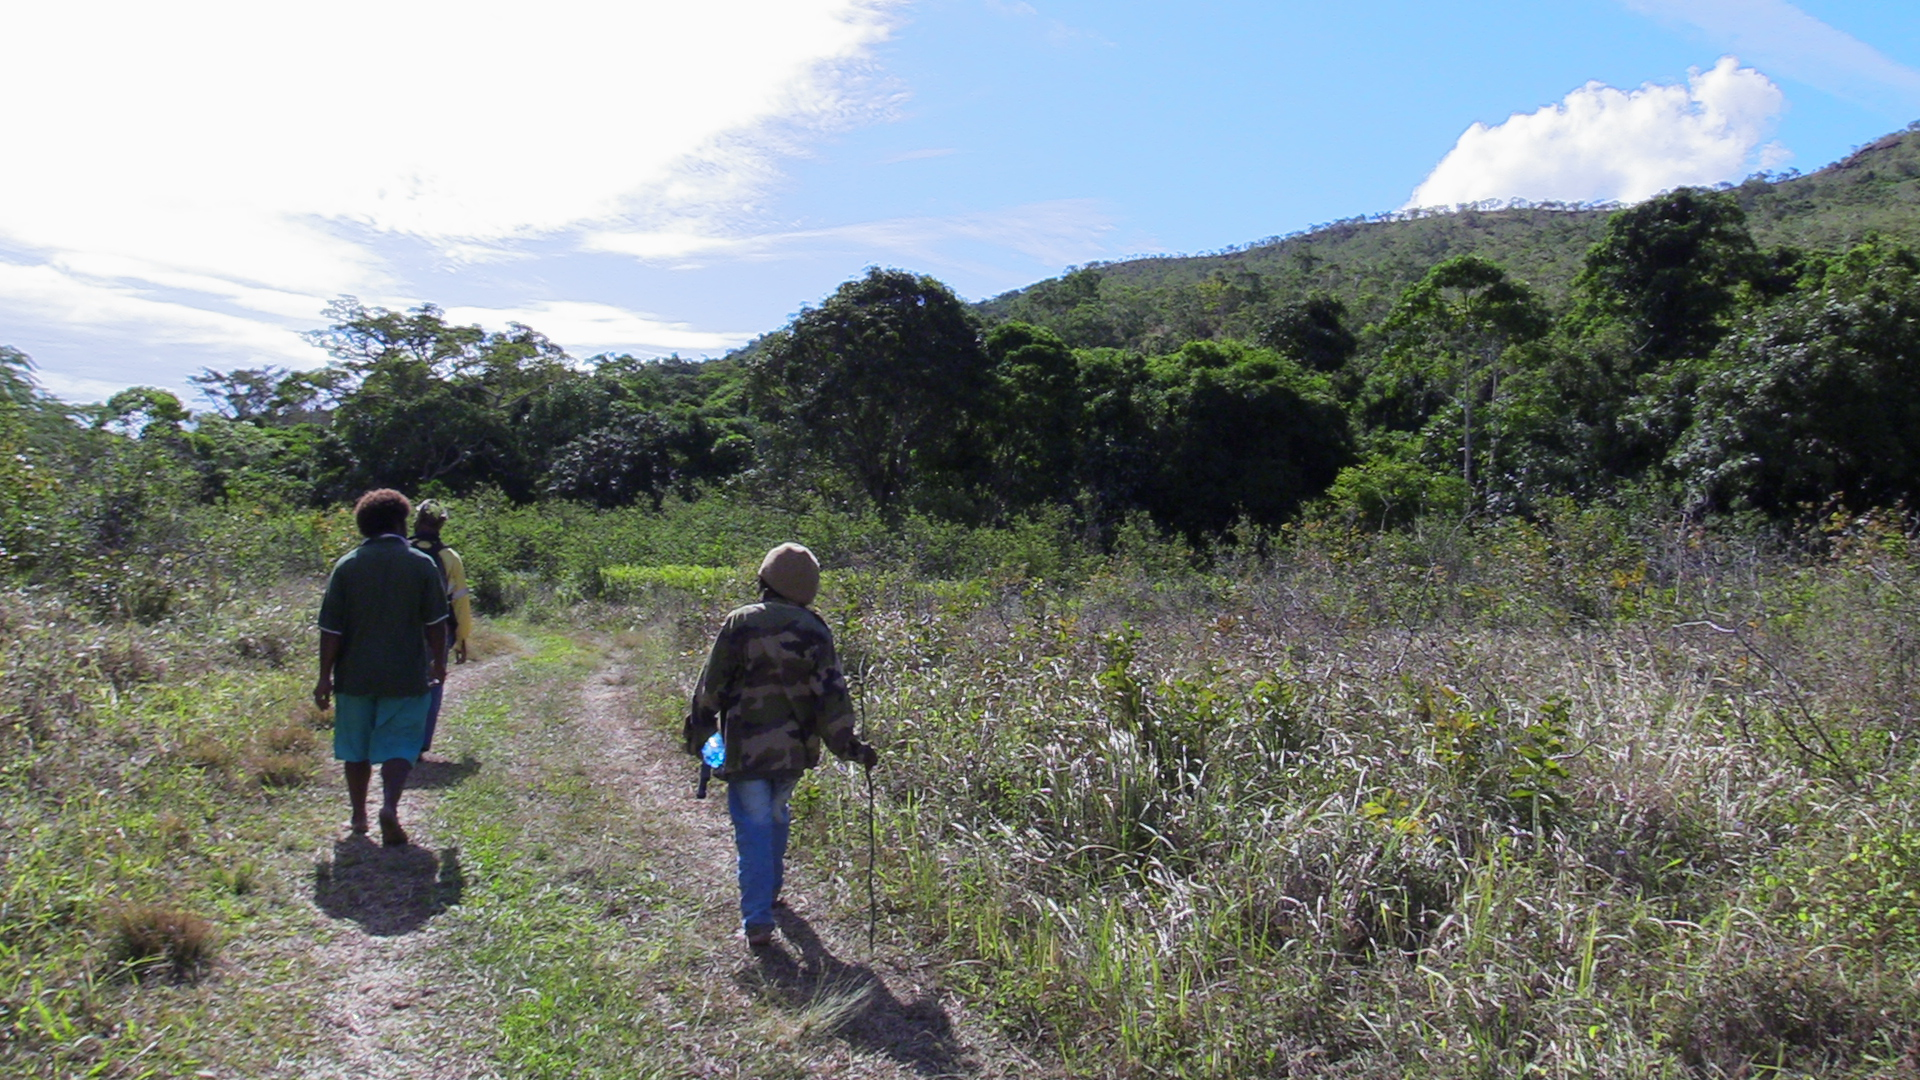
\includegraphics[width=\linewidth]{figures/bande}
	\caption{Mr.\ Pei and Mr.\ Kalène on the path to Wanaa}
\end{figure}

